% lecture6_ro.tex -- GENERATED by build_L6.py from L6_numbers.json; do not edit by hand.
\documentclass[10pt,aspectratio=169,t]{beamer}
% =============================================================================
% emqa_preamble.tex -- shared Beamer preamble of Energy Markets Quantitative Analysis (EMQA)
% Used by every lecture: lectures/Lk/lecturek.tex does
%   \documentclass[10pt,aspectratio=169,t]{beamer}
%   % =============================================================================
% emqa_preamble.tex -- shared Beamer preamble of Energy Markets Quantitative Analysis (EMQA)
% Used by every lecture: lectures/Lk/lecturek.tex does
%   \documentclass[10pt,aspectratio=169,t]{beamer}
%   % =============================================================================
% emqa_preamble.tex -- shared Beamer preamble of Energy Markets Quantitative Analysis (EMQA)
% Used by every lecture: lectures/Lk/lecturek.tex does
%   \documentclass[10pt,aspectratio=169,t]{beamer}
%   \input{../common/emqa_preamble}
%   \emqalecture{k}{Lecture title}
% Logos live in lectures/common/logos/, charts in lectures/Lk/charts/.
% Do NOT add \hfuzz / \vfuzz / \hbadness here: overfull boxes must be fixed, not hidden.
% =============================================================================

\usetheme{default}
\setbeamersize{text margin left=7mm, text margin right=7mm}

% ---------------------------------------------------------------- packages
\usepackage[utf8]{inputenc}
\usepackage[T1]{fontenc}
\usepackage{lmodern}
\usepackage{amsmath, amssymb}
\usepackage{mathtools}
\usepackage{bm}
\usepackage{tikz}
\usetikzlibrary{arrows.meta, positioning, calc, shapes.misc}
\usepackage{booktabs}
\usepackage{array}
\usepackage{graphicx}
\usepackage{colortbl}
\usepackage{xcolor}
\usepackage{multicol}
\hypersetup{colorlinks=true, linkcolor=MainBlue, urlcolor=MainBlue, citecolor=MainBlue}
\graphicspath{{../common/logos/}}   % charts are included with their language folder: charts/en/, charts/ro/

% ---------------------------------------------------------------- colours
\definecolor{MainBlue}{RGB}{26, 58, 110}
\definecolor{IDAred}{RGB}{205, 0, 0}
\definecolor{DarkGray}{RGB}{51, 51, 51}
\definecolor{FooterGray}{RGB}{100, 100, 100}
\definecolor{BlockGray}{RGB}{236, 238, 242}
\definecolor{KeynoteGray}{RGB}{218, 218, 218}
\definecolor{Crimson}{RGB}{190, 40, 50}
\definecolor{Forest}{RGB}{30, 110, 50}
\definecolor{Bitter}{RGB}{214, 150, 20}
% chart palette (same hex values as lectures/common/emqa_plot.py)
\definecolor{SerRO}{HTML}{2A78D6}
\definecolor{SerDE}{HTML}{EB6834}
\definecolor{SerHU}{HTML}{1BAF7A}
\definecolor{SerBG}{HTML}{EDA100}

\setbeamertemplate{background}{%
  \begin{tikzpicture}[remember picture, overlay]
    \shade[shading=axis, shading angle=315, top color=white, bottom color=KeynoteGray]
      (current page.south west) rectangle (current page.north east);
  \end{tikzpicture}}
\setbeamercolor{background canvas}{bg=}
\setbeamercolor{structure}{fg=MainBlue}
\setbeamercolor{normal text}{fg=DarkGray}
\setbeamercolor{title}{fg=IDAred}
\setbeamercolor{frametitle}{fg=IDAred, bg=}
\setbeamercolor{block title}{bg=MainBlue, fg=white}
\setbeamercolor{block body}{bg=BlockGray, fg=DarkGray}
\setbeamercolor{block title alerted}{bg=Crimson, fg=white}
\setbeamercolor{block body alerted}{bg=Crimson!7, fg=DarkGray}
\setbeamercolor{block title example}{bg=Forest, fg=white}
\setbeamercolor{block body example}{bg=Forest!7, fg=DarkGray}
\setbeamercolor{item}{fg=MainBlue}
\setbeamerfont{frametitle}{size=\large, series=\bfseries}
\setbeamerfont{block title}{size=\small, series=\bfseries}
\setbeamertemplate{blocks}[rounded][shadow=false]
\setbeamertemplate{itemize item}{\color{MainBlue}$\boxdot$}
\setbeamertemplate{itemize subitem}{\color{MainBlue}\scriptsize$\blacktriangleright$}
% compact two-level lists: level 1 = main point, level 2 = details (no text outside bullets)
\setbeamerfont{itemize/enumerate subbody}{size=\footnotesize}
\setlength{\leftmargini}{1.1em}
\setlength{\leftmarginii}{1.1em}
\setbeamertemplate{itemize/enumerate body begin}{\setlength{\topsep}{0pt}\setlength{\partopsep}{0pt}\setlength{\parskip}{0pt}}
\setbeamertemplate{itemize/enumerate subbody begin}{\setlength{\topsep}{0pt}\setlength{\partopsep}{0pt}\setlength{\itemsep}{0pt}\vspace{-0.4ex}}

\setbeamertemplate{enumerate item}{\color{MainBlue}\insertenumlabel.}
\setlength{\leftmargini}{1.3em}
\setlength{\leftmarginii}{1.2em}
\setbeamertemplate{navigation symbols}{}
\setbeamertemplate{section in toc}{\color{MainBlue}$\blacktriangleright$~\inserttocsection}
\setbeamertemplate{caption}{\raggedright\insertcaption\par}
% frame subtitle = precise citation line under the claim title (Weron style)
\setbeamerfont{framesubtitle}{size=\footnotesize}
\setbeamercolor{framesubtitle}{fg=FooterGray}
% outline that reappears at every section with the current section highlighted
\setbeamertemplate{section in toc shaded}[default][35]
\setbeamertemplate{subsection in toc shaded}[default][35]
\setbeamertemplate{subsection in toc}{\leavevmode\leftskip=2.2em\color{DarkGray}\small\inserttocsubsection\par}
\AtBeginSection[]{{\begin{frame}{\txtoutline}\vspace{2mm}\small
  \tableofcontents[currentsection,hideothersubsections]\end{frame}}}

% ---------------------------------------------------------------- head and foot
\setbeamertemplate{headline}{%
  \vskip10pt%
  \hbox to \paperwidth{\hskip0.5cm%
    {\small\color{FooterGray}\renewcommand{\hyperlink}[2]{##2}\insertsectionhead}%
    \hfill\textcolor{FooterGray}{\small\insertframenumber}\hskip0.5cm}%
  \vskip4pt{\color{FooterGray}\hrule height 0.4pt}}
% footer as in the other courses (MFM, SFM): course name on the left, small sparkline on the right
\setbeamertemplate{footline}{%
  {\color{FooterGray}\hrule height 0.4pt}\vskip4pt%
  \hbox to \paperwidth{\hskip0.5cm%
    \textcolor{FooterGray}{\small\txtcourse}%
    \hfill\raisebox{-0.1em}{\begin{tikzpicture}[x=0.08em, y=0.08em, line width=0.4pt]
      \draw[FooterGray] (0,3) -- (1,4) -- (2,3.5) -- (3,5) -- (4,4) -- (5,6) -- (6,5.5) -- (7,4) -- (8,5) -- (9,7) -- (10,6) -- (11,5) -- (12,6.5) -- (13,8) -- (14,7) -- (15,6) -- (16,7.5) -- (17,9) -- (18,8) -- (19,7) -- (20,8.5) -- (21,10) -- (22,9) -- (23,8) -- (24,9.5);
    \end{tikzpicture}}\hskip0.5cm}%
  \vskip6pt}

% ---------------------------------------------------------------- title page
\defbeamertemplate*{title page}{emqa}[1][]{%
  \vspace{0.15cm}
  \begin{center}
    \href{https://www.ase.ro}{
\includegraphics[height=0.9cm]{ase_logo.png}}\hspace{0.3cm}%
    \href{https://ipe.ro/new}{
\includegraphics[height=0.9cm]{acad_logo.png}}\hspace{0.3cm}%
    \href{https://theida.net}{
\includegraphics[height=0.9cm]{ida_logo.png}}\hspace{0.3cm}%
    \href{https://blockchain-research-center.com}{
\includegraphics[height=0.9cm]{brc_logo.png}}\hspace{0.3cm}%
    \href{https://www.ai4efin.ase.ro}{
\includegraphics[height=0.9cm]{ai4efin_logo.png}}\hspace{0.3cm}%
    \href{https://www.digital-finance-msca.com}{
\includegraphics[height=0.9cm]{msca_logo.png}}%
  \end{center}
  \vspace{0.45cm}
  \begin{center}
    \begin{minipage}{0.1\textwidth}\centering
      \href{https://quantlet.com}{
\includegraphics[height=0.9cm]{ql_logo.png}}\end{minipage}%
    \begin{minipage}{0.78\textwidth}\centering
      {\Large\bfseries\usebeamercolor[fg]{title}\inserttitle}\par\vspace{0.25cm}
      {\large\usebeamercolor[fg]{title}\insertsubtitle}\end{minipage}%
    \begin{minipage}{0.1\textwidth}\centering
      \href{https://quantinar.com}{
\includegraphics[height=0.9cm]{qr_logo.png}}\end{minipage}
  \end{center}
  \vfill
  \hspace{0.4cm}{\bfseries\insertauthor}\par\vspace{0.12cm}
  \hspace{0.4cm}\begin{minipage}[t]{0.92\textwidth}\raggedright\footnotesize\insertinstitute\end{minipage}
  \par\vspace{0.4cm}}

% ---------------------------------------------------------------- lecture metadata
\newcommand{\emqashort}{}
\newcommand{\emqanb}{notebooks}
\newcommand{\emqarepo}{https://github.com/danpele/EMQA/tree/main}
% language-dependent labels (English default; \emqaromanian switches to Romanian, call it before \emqalecture)
\newcommand{\txtcourse}{Energy Markets Quantitative Analysis}
\newcommand{\txtlecture}{Lecture}
\newcommand{\txtoutline}{Outline}
\newcommand{\txtintuition}{In one sentence:}
\newcommand{\txtjob}{In practice:}
\newcommand{\txttry}{Experiment yourself:}
\newcommand{\txtwhere}{where}
\newcommand{\txtsim}{SIMULATED DATA (teaching illustration)}
\newcommand{\txtnbsuffix}{}
\newcommand{\txtinstitute}{Bucharest University of Economic Studies, Department of Statistics and Econometrics\\
    Romanian Academy, Institute for Economic Forecasting\\
    IDA Institute Digital Assets \textbullet\ AI4EFin \textbullet\ MSCA Digital Finance}
\newcommand{\emqaromanian}{%
  \renewcommand{\txtcourse}{Analiza cantitativă a piețelor de energie}%
  \renewcommand{\txtlecture}{Cursul}%
  \renewcommand{\txtoutline}{Cuprins}%
  \renewcommand{\txtintuition}{Pe scurt:}%
  \renewcommand{\txtjob}{În practică:}%
  \renewcommand{\txttry}{Exercițiu practic:}%
  \renewcommand{\txtwhere}{unde}%
  \renewcommand{\txtsim}{DATE SIMULATE (doar pentru ilustrare)}%
  \renewcommand{\txtnbsuffix}{\string_ro}%
  \renewcommand{\txtinstitute}{Academia de Studii Economice din București, Departamentul de Statistică și Econometrie\\
    Academia Română, Institutul de Prognoză Economică\\
    IDA Institute Digital Assets \textbullet\ AI4EFin \textbullet\ MSCA Digital Finance}}
\newcommand{\emqalecture}[2]{%
  \renewcommand{\emqashort}{\txtlecture\ #1}%
  \renewcommand{\emqanb}{notebooks/L#1\string_notebook\txtnbsuffix.ipynb}%
  \title[EMQA]{\txtcourse}%
  \subtitle{\txtlecture\ #1: #2}%
  \author{Prof.\ dr.\ Daniel Traian PELE}%
  \institute{\txtinstitute}%
  \date{}}

% ---------------------------------------------------------------- teaching blocks (MBA clarity rule)
% \intuition{one plain sentence}  ->  formula with every symbol defined  ->  real-data example  ->  \manager{one line}
\newcommand{\intuition}[1]{\begin{itemize}\item {\color{MainBlue}\textbf{\txtintuition}}~#1\end{itemize}\vspace{0.6mm}}
\newcommand{\manager}[1]{\colorbox{Forest!10}{\parbox{\dimexpr\linewidth-2\fboxsep\relax}{\footnotesize
  \begin{itemize}\setlength{\itemsep}{0pt}\item \textbf{\color{Forest}\txtjob}~#1\end{itemize}}}}
% Experiment yourself: pointer to the matching notebook section
\newcommand{\tryit}[1]{{\scriptsize\href{\emqarepo/\emqanb}{%
  \raisebox{-0.15em}{
\includegraphics[height=0.85em]{ql_logo.png}}\,\textbf{\txttry}~\color{MainBlue}#1}}}
% bottom row: manager line (left) + experiment pointer (right), pinned to the bottom of the frame
\newcommand{\bottomrow}[2]{\par\vfill\noindent\begin{minipage}[b]{0.72\linewidth}#1\end{minipage}\hfill
  \begin{minipage}[b]{0.26\linewidth}\raggedleft #2\end{minipage}\par\vspace{0.5mm}}
\newcommand{\where}[1]{{\footnotesize\textbf{\txtwhere}~#1\par}}

% ---------------------------------------------------------------- helpers
% chart source line under a figure: \chartsource{Source ...; period ...}
\newcommand{\chartsource}[1]{\par\vspace{1pt}{\scriptsize\color{FooterGray}#1\par}}
% link to code: \quantlet{label}{path inside the repo}
\newcommand{\quantlet}[2]{\par\vspace{1pt}\hfill\href{\emqarepo/#2}{%
  \raisebox{-0.15em}{
\includegraphics[height=0.75em]{ql_logo.png}}\textcolor{MainBlue}{\scriptsize\ #1}}}
\newcommand{\simlabel}{\colorbox{Crimson!12}{\scriptsize\bfseries\color{Crimson}\txtsim}}
\newcommand{\E}{\mathbb{E}}
\newcommand{\Var}{\operatorname{Var}}
\newcommand{\Cov}{\operatorname{Cov}}
\newcommand{\Corr}{\operatorname{Corr}}
\newcommand{\asinh}{\operatorname{asinh}}
\newcommand{\iid}{\overset{\text{i.i.d.}}{\sim}}
\newcommand{\EUR}{EUR}

%   \emqalecture{k}{Lecture title}
% Logos live in lectures/common/logos/, charts in lectures/Lk/charts/.
% Do NOT add \hfuzz / \vfuzz / \hbadness here: overfull boxes must be fixed, not hidden.
% =============================================================================

\usetheme{default}
\setbeamersize{text margin left=7mm, text margin right=7mm}

% ---------------------------------------------------------------- packages
\usepackage[utf8]{inputenc}
\usepackage[T1]{fontenc}
\usepackage{lmodern}
\usepackage{amsmath, amssymb}
\usepackage{mathtools}
\usepackage{bm}
\usepackage{tikz}
\usetikzlibrary{arrows.meta, positioning, calc, shapes.misc}
\usepackage{booktabs}
\usepackage{array}
\usepackage{graphicx}
\usepackage{colortbl}
\usepackage{xcolor}
\usepackage{multicol}
\hypersetup{colorlinks=true, linkcolor=MainBlue, urlcolor=MainBlue, citecolor=MainBlue}
\graphicspath{{../common/logos/}}   % charts are included with their language folder: charts/en/, charts/ro/

% ---------------------------------------------------------------- colours
\definecolor{MainBlue}{RGB}{26, 58, 110}
\definecolor{IDAred}{RGB}{205, 0, 0}
\definecolor{DarkGray}{RGB}{51, 51, 51}
\definecolor{FooterGray}{RGB}{100, 100, 100}
\definecolor{BlockGray}{RGB}{236, 238, 242}
\definecolor{KeynoteGray}{RGB}{218, 218, 218}
\definecolor{Crimson}{RGB}{190, 40, 50}
\definecolor{Forest}{RGB}{30, 110, 50}
\definecolor{Bitter}{RGB}{214, 150, 20}
% chart palette (same hex values as lectures/common/emqa_plot.py)
\definecolor{SerRO}{HTML}{2A78D6}
\definecolor{SerDE}{HTML}{EB6834}
\definecolor{SerHU}{HTML}{1BAF7A}
\definecolor{SerBG}{HTML}{EDA100}

\setbeamertemplate{background}{%
  \begin{tikzpicture}[remember picture, overlay]
    \shade[shading=axis, shading angle=315, top color=white, bottom color=KeynoteGray]
      (current page.south west) rectangle (current page.north east);
  \end{tikzpicture}}
\setbeamercolor{background canvas}{bg=}
\setbeamercolor{structure}{fg=MainBlue}
\setbeamercolor{normal text}{fg=DarkGray}
\setbeamercolor{title}{fg=IDAred}
\setbeamercolor{frametitle}{fg=IDAred, bg=}
\setbeamercolor{block title}{bg=MainBlue, fg=white}
\setbeamercolor{block body}{bg=BlockGray, fg=DarkGray}
\setbeamercolor{block title alerted}{bg=Crimson, fg=white}
\setbeamercolor{block body alerted}{bg=Crimson!7, fg=DarkGray}
\setbeamercolor{block title example}{bg=Forest, fg=white}
\setbeamercolor{block body example}{bg=Forest!7, fg=DarkGray}
\setbeamercolor{item}{fg=MainBlue}
\setbeamerfont{frametitle}{size=\large, series=\bfseries}
\setbeamerfont{block title}{size=\small, series=\bfseries}
\setbeamertemplate{blocks}[rounded][shadow=false]
\setbeamertemplate{itemize item}{\color{MainBlue}$\boxdot$}
\setbeamertemplate{itemize subitem}{\color{MainBlue}\scriptsize$\blacktriangleright$}
% compact two-level lists: level 1 = main point, level 2 = details (no text outside bullets)
\setbeamerfont{itemize/enumerate subbody}{size=\footnotesize}
\setlength{\leftmargini}{1.1em}
\setlength{\leftmarginii}{1.1em}
\setbeamertemplate{itemize/enumerate body begin}{\setlength{\topsep}{0pt}\setlength{\partopsep}{0pt}\setlength{\parskip}{0pt}}
\setbeamertemplate{itemize/enumerate subbody begin}{\setlength{\topsep}{0pt}\setlength{\partopsep}{0pt}\setlength{\itemsep}{0pt}\vspace{-0.4ex}}

\setbeamertemplate{enumerate item}{\color{MainBlue}\insertenumlabel.}
\setlength{\leftmargini}{1.3em}
\setlength{\leftmarginii}{1.2em}
\setbeamertemplate{navigation symbols}{}
\setbeamertemplate{section in toc}{\color{MainBlue}$\blacktriangleright$~\inserttocsection}
\setbeamertemplate{caption}{\raggedright\insertcaption\par}
% frame subtitle = precise citation line under the claim title (Weron style)
\setbeamerfont{framesubtitle}{size=\footnotesize}
\setbeamercolor{framesubtitle}{fg=FooterGray}
% outline that reappears at every section with the current section highlighted
\setbeamertemplate{section in toc shaded}[default][35]
\setbeamertemplate{subsection in toc shaded}[default][35]
\setbeamertemplate{subsection in toc}{\leavevmode\leftskip=2.2em\color{DarkGray}\small\inserttocsubsection\par}
\AtBeginSection[]{{\begin{frame}{\txtoutline}\vspace{2mm}\small
  \tableofcontents[currentsection,hideothersubsections]\end{frame}}}

% ---------------------------------------------------------------- head and foot
\setbeamertemplate{headline}{%
  \vskip10pt%
  \hbox to \paperwidth{\hskip0.5cm%
    {\small\color{FooterGray}\renewcommand{\hyperlink}[2]{##2}\insertsectionhead}%
    \hfill\textcolor{FooterGray}{\small\insertframenumber}\hskip0.5cm}%
  \vskip4pt{\color{FooterGray}\hrule height 0.4pt}}
% footer as in the other courses (MFM, SFM): course name on the left, small sparkline on the right
\setbeamertemplate{footline}{%
  {\color{FooterGray}\hrule height 0.4pt}\vskip4pt%
  \hbox to \paperwidth{\hskip0.5cm%
    \textcolor{FooterGray}{\small\txtcourse}%
    \hfill\raisebox{-0.1em}{\begin{tikzpicture}[x=0.08em, y=0.08em, line width=0.4pt]
      \draw[FooterGray] (0,3) -- (1,4) -- (2,3.5) -- (3,5) -- (4,4) -- (5,6) -- (6,5.5) -- (7,4) -- (8,5) -- (9,7) -- (10,6) -- (11,5) -- (12,6.5) -- (13,8) -- (14,7) -- (15,6) -- (16,7.5) -- (17,9) -- (18,8) -- (19,7) -- (20,8.5) -- (21,10) -- (22,9) -- (23,8) -- (24,9.5);
    \end{tikzpicture}}\hskip0.5cm}%
  \vskip6pt}

% ---------------------------------------------------------------- title page
\defbeamertemplate*{title page}{emqa}[1][]{%
  \vspace{0.15cm}
  \begin{center}
    \href{https://www.ase.ro}{
\includegraphics[height=0.9cm]{ase_logo.png}}\hspace{0.3cm}%
    \href{https://ipe.ro/new}{
\includegraphics[height=0.9cm]{acad_logo.png}}\hspace{0.3cm}%
    \href{https://theida.net}{
\includegraphics[height=0.9cm]{ida_logo.png}}\hspace{0.3cm}%
    \href{https://blockchain-research-center.com}{
\includegraphics[height=0.9cm]{brc_logo.png}}\hspace{0.3cm}%
    \href{https://www.ai4efin.ase.ro}{
\includegraphics[height=0.9cm]{ai4efin_logo.png}}\hspace{0.3cm}%
    \href{https://www.digital-finance-msca.com}{
\includegraphics[height=0.9cm]{msca_logo.png}}%
  \end{center}
  \vspace{0.45cm}
  \begin{center}
    \begin{minipage}{0.1\textwidth}\centering
      \href{https://quantlet.com}{
\includegraphics[height=0.9cm]{ql_logo.png}}\end{minipage}%
    \begin{minipage}{0.78\textwidth}\centering
      {\Large\bfseries\usebeamercolor[fg]{title}\inserttitle}\par\vspace{0.25cm}
      {\large\usebeamercolor[fg]{title}\insertsubtitle}\end{minipage}%
    \begin{minipage}{0.1\textwidth}\centering
      \href{https://quantinar.com}{
\includegraphics[height=0.9cm]{qr_logo.png}}\end{minipage}
  \end{center}
  \vfill
  \hspace{0.4cm}{\bfseries\insertauthor}\par\vspace{0.12cm}
  \hspace{0.4cm}\begin{minipage}[t]{0.92\textwidth}\raggedright\footnotesize\insertinstitute\end{minipage}
  \par\vspace{0.4cm}}

% ---------------------------------------------------------------- lecture metadata
\newcommand{\emqashort}{}
\newcommand{\emqanb}{notebooks}
\newcommand{\emqarepo}{https://github.com/danpele/EMQA/tree/main}
% language-dependent labels (English default; \emqaromanian switches to Romanian, call it before \emqalecture)
\newcommand{\txtcourse}{Energy Markets Quantitative Analysis}
\newcommand{\txtlecture}{Lecture}
\newcommand{\txtoutline}{Outline}
\newcommand{\txtintuition}{In one sentence:}
\newcommand{\txtjob}{In practice:}
\newcommand{\txttry}{Experiment yourself:}
\newcommand{\txtwhere}{where}
\newcommand{\txtsim}{SIMULATED DATA (teaching illustration)}
\newcommand{\txtnbsuffix}{}
\newcommand{\txtinstitute}{Bucharest University of Economic Studies, Department of Statistics and Econometrics\\
    Romanian Academy, Institute for Economic Forecasting\\
    IDA Institute Digital Assets \textbullet\ AI4EFin \textbullet\ MSCA Digital Finance}
\newcommand{\emqaromanian}{%
  \renewcommand{\txtcourse}{Analiza cantitativă a piețelor de energie}%
  \renewcommand{\txtlecture}{Cursul}%
  \renewcommand{\txtoutline}{Cuprins}%
  \renewcommand{\txtintuition}{Pe scurt:}%
  \renewcommand{\txtjob}{În practică:}%
  \renewcommand{\txttry}{Exercițiu practic:}%
  \renewcommand{\txtwhere}{unde}%
  \renewcommand{\txtsim}{DATE SIMULATE (doar pentru ilustrare)}%
  \renewcommand{\txtnbsuffix}{\string_ro}%
  \renewcommand{\txtinstitute}{Academia de Studii Economice din București, Departamentul de Statistică și Econometrie\\
    Academia Română, Institutul de Prognoză Economică\\
    IDA Institute Digital Assets \textbullet\ AI4EFin \textbullet\ MSCA Digital Finance}}
\newcommand{\emqalecture}[2]{%
  \renewcommand{\emqashort}{\txtlecture\ #1}%
  \renewcommand{\emqanb}{notebooks/L#1\string_notebook\txtnbsuffix.ipynb}%
  \title[EMQA]{\txtcourse}%
  \subtitle{\txtlecture\ #1: #2}%
  \author{Prof.\ dr.\ Daniel Traian PELE}%
  \institute{\txtinstitute}%
  \date{}}

% ---------------------------------------------------------------- teaching blocks (MBA clarity rule)
% \intuition{one plain sentence}  ->  formula with every symbol defined  ->  real-data example  ->  \manager{one line}
\newcommand{\intuition}[1]{\begin{itemize}\item {\color{MainBlue}\textbf{\txtintuition}}~#1\end{itemize}\vspace{0.6mm}}
\newcommand{\manager}[1]{\colorbox{Forest!10}{\parbox{\dimexpr\linewidth-2\fboxsep\relax}{\footnotesize
  \begin{itemize}\setlength{\itemsep}{0pt}\item \textbf{\color{Forest}\txtjob}~#1\end{itemize}}}}
% Experiment yourself: pointer to the matching notebook section
\newcommand{\tryit}[1]{{\scriptsize\href{\emqarepo/\emqanb}{%
  \raisebox{-0.15em}{
\includegraphics[height=0.85em]{ql_logo.png}}\,\textbf{\txttry}~\color{MainBlue}#1}}}
% bottom row: manager line (left) + experiment pointer (right), pinned to the bottom of the frame
\newcommand{\bottomrow}[2]{\par\vfill\noindent\begin{minipage}[b]{0.72\linewidth}#1\end{minipage}\hfill
  \begin{minipage}[b]{0.26\linewidth}\raggedleft #2\end{minipage}\par\vspace{0.5mm}}
\newcommand{\where}[1]{{\footnotesize\textbf{\txtwhere}~#1\par}}

% ---------------------------------------------------------------- helpers
% chart source line under a figure: \chartsource{Source ...; period ...}
\newcommand{\chartsource}[1]{\par\vspace{1pt}{\scriptsize\color{FooterGray}#1\par}}
% link to code: \quantlet{label}{path inside the repo}
\newcommand{\quantlet}[2]{\par\vspace{1pt}\hfill\href{\emqarepo/#2}{%
  \raisebox{-0.15em}{
\includegraphics[height=0.75em]{ql_logo.png}}\textcolor{MainBlue}{\scriptsize\ #1}}}
\newcommand{\simlabel}{\colorbox{Crimson!12}{\scriptsize\bfseries\color{Crimson}\txtsim}}
\newcommand{\E}{\mathbb{E}}
\newcommand{\Var}{\operatorname{Var}}
\newcommand{\Cov}{\operatorname{Cov}}
\newcommand{\Corr}{\operatorname{Corr}}
\newcommand{\asinh}{\operatorname{asinh}}
\newcommand{\iid}{\overset{\text{i.i.d.}}{\sim}}
\newcommand{\EUR}{EUR}

%   \emqalecture{k}{Lecture title}
% Logos live in lectures/common/logos/, charts in lectures/Lk/charts/.
% Do NOT add \hfuzz / \vfuzz / \hbadness here: overfull boxes must be fixed, not hidden.
% =============================================================================

\usetheme{default}
\setbeamersize{text margin left=7mm, text margin right=7mm}

% ---------------------------------------------------------------- packages
\usepackage[utf8]{inputenc}
\usepackage[T1]{fontenc}
\usepackage{lmodern}
\usepackage{amsmath, amssymb}
\usepackage{mathtools}
\usepackage{bm}
\usepackage{tikz}
\usetikzlibrary{arrows.meta, positioning, calc, shapes.misc}
\usepackage{booktabs}
\usepackage{array}
\usepackage{graphicx}
\usepackage{colortbl}
\usepackage{xcolor}
\usepackage{multicol}
\hypersetup{colorlinks=true, linkcolor=MainBlue, urlcolor=MainBlue, citecolor=MainBlue}
\graphicspath{{../common/logos/}}   % charts are included with their language folder: charts/en/, charts/ro/

% ---------------------------------------------------------------- colours
\definecolor{MainBlue}{RGB}{26, 58, 110}
\definecolor{IDAred}{RGB}{205, 0, 0}
\definecolor{DarkGray}{RGB}{51, 51, 51}
\definecolor{FooterGray}{RGB}{100, 100, 100}
\definecolor{BlockGray}{RGB}{236, 238, 242}
\definecolor{KeynoteGray}{RGB}{218, 218, 218}
\definecolor{Crimson}{RGB}{190, 40, 50}
\definecolor{Forest}{RGB}{30, 110, 50}
\definecolor{Bitter}{RGB}{214, 150, 20}
% chart palette (same hex values as lectures/common/emqa_plot.py)
\definecolor{SerRO}{HTML}{2A78D6}
\definecolor{SerDE}{HTML}{EB6834}
\definecolor{SerHU}{HTML}{1BAF7A}
\definecolor{SerBG}{HTML}{EDA100}

\setbeamertemplate{background}{%
  \begin{tikzpicture}[remember picture, overlay]
    \shade[shading=axis, shading angle=315, top color=white, bottom color=KeynoteGray]
      (current page.south west) rectangle (current page.north east);
  \end{tikzpicture}}
\setbeamercolor{background canvas}{bg=}
\setbeamercolor{structure}{fg=MainBlue}
\setbeamercolor{normal text}{fg=DarkGray}
\setbeamercolor{title}{fg=IDAred}
\setbeamercolor{frametitle}{fg=IDAred, bg=}
\setbeamercolor{block title}{bg=MainBlue, fg=white}
\setbeamercolor{block body}{bg=BlockGray, fg=DarkGray}
\setbeamercolor{block title alerted}{bg=Crimson, fg=white}
\setbeamercolor{block body alerted}{bg=Crimson!7, fg=DarkGray}
\setbeamercolor{block title example}{bg=Forest, fg=white}
\setbeamercolor{block body example}{bg=Forest!7, fg=DarkGray}
\setbeamercolor{item}{fg=MainBlue}
\setbeamerfont{frametitle}{size=\large, series=\bfseries}
\setbeamerfont{block title}{size=\small, series=\bfseries}
\setbeamertemplate{blocks}[rounded][shadow=false]
\setbeamertemplate{itemize item}{\color{MainBlue}$\boxdot$}
\setbeamertemplate{itemize subitem}{\color{MainBlue}\scriptsize$\blacktriangleright$}
% compact two-level lists: level 1 = main point, level 2 = details (no text outside bullets)
\setbeamerfont{itemize/enumerate subbody}{size=\footnotesize}
\setlength{\leftmargini}{1.1em}
\setlength{\leftmarginii}{1.1em}
\setbeamertemplate{itemize/enumerate body begin}{\setlength{\topsep}{0pt}\setlength{\partopsep}{0pt}\setlength{\parskip}{0pt}}
\setbeamertemplate{itemize/enumerate subbody begin}{\setlength{\topsep}{0pt}\setlength{\partopsep}{0pt}\setlength{\itemsep}{0pt}\vspace{-0.4ex}}

\setbeamertemplate{enumerate item}{\color{MainBlue}\insertenumlabel.}
\setlength{\leftmargini}{1.3em}
\setlength{\leftmarginii}{1.2em}
\setbeamertemplate{navigation symbols}{}
\setbeamertemplate{section in toc}{\color{MainBlue}$\blacktriangleright$~\inserttocsection}
\setbeamertemplate{caption}{\raggedright\insertcaption\par}
% frame subtitle = precise citation line under the claim title (Weron style)
\setbeamerfont{framesubtitle}{size=\footnotesize}
\setbeamercolor{framesubtitle}{fg=FooterGray}
% outline that reappears at every section with the current section highlighted
\setbeamertemplate{section in toc shaded}[default][35]
\setbeamertemplate{subsection in toc shaded}[default][35]
\setbeamertemplate{subsection in toc}{\leavevmode\leftskip=2.2em\color{DarkGray}\small\inserttocsubsection\par}
\AtBeginSection[]{{\begin{frame}{\txtoutline}\vspace{2mm}\small
  \tableofcontents[currentsection,hideothersubsections]\end{frame}}}

% ---------------------------------------------------------------- head and foot
\setbeamertemplate{headline}{%
  \vskip10pt%
  \hbox to \paperwidth{\hskip0.5cm%
    {\small\color{FooterGray}\renewcommand{\hyperlink}[2]{##2}\insertsectionhead}%
    \hfill\textcolor{FooterGray}{\small\insertframenumber}\hskip0.5cm}%
  \vskip4pt{\color{FooterGray}\hrule height 0.4pt}}
% footer as in the other courses (MFM, SFM): course name on the left, small sparkline on the right
\setbeamertemplate{footline}{%
  {\color{FooterGray}\hrule height 0.4pt}\vskip4pt%
  \hbox to \paperwidth{\hskip0.5cm%
    \textcolor{FooterGray}{\small\txtcourse}%
    \hfill\raisebox{-0.1em}{\begin{tikzpicture}[x=0.08em, y=0.08em, line width=0.4pt]
      \draw[FooterGray] (0,3) -- (1,4) -- (2,3.5) -- (3,5) -- (4,4) -- (5,6) -- (6,5.5) -- (7,4) -- (8,5) -- (9,7) -- (10,6) -- (11,5) -- (12,6.5) -- (13,8) -- (14,7) -- (15,6) -- (16,7.5) -- (17,9) -- (18,8) -- (19,7) -- (20,8.5) -- (21,10) -- (22,9) -- (23,8) -- (24,9.5);
    \end{tikzpicture}}\hskip0.5cm}%
  \vskip6pt}

% ---------------------------------------------------------------- title page
\defbeamertemplate*{title page}{emqa}[1][]{%
  \vspace{0.15cm}
  \begin{center}
    \href{https://www.ase.ro}{
\includegraphics[height=0.9cm]{ase_logo.png}}\hspace{0.3cm}%
    \href{https://ipe.ro/new}{
\includegraphics[height=0.9cm]{acad_logo.png}}\hspace{0.3cm}%
    \href{https://theida.net}{
\includegraphics[height=0.9cm]{ida_logo.png}}\hspace{0.3cm}%
    \href{https://blockchain-research-center.com}{
\includegraphics[height=0.9cm]{brc_logo.png}}\hspace{0.3cm}%
    \href{https://www.ai4efin.ase.ro}{
\includegraphics[height=0.9cm]{ai4efin_logo.png}}\hspace{0.3cm}%
    \href{https://www.digital-finance-msca.com}{
\includegraphics[height=0.9cm]{msca_logo.png}}%
  \end{center}
  \vspace{0.45cm}
  \begin{center}
    \begin{minipage}{0.1\textwidth}\centering
      \href{https://quantlet.com}{
\includegraphics[height=0.9cm]{ql_logo.png}}\end{minipage}%
    \begin{minipage}{0.78\textwidth}\centering
      {\Large\bfseries\usebeamercolor[fg]{title}\inserttitle}\par\vspace{0.25cm}
      {\large\usebeamercolor[fg]{title}\insertsubtitle}\end{minipage}%
    \begin{minipage}{0.1\textwidth}\centering
      \href{https://quantinar.com}{
\includegraphics[height=0.9cm]{qr_logo.png}}\end{minipage}
  \end{center}
  \vfill
  \hspace{0.4cm}{\bfseries\insertauthor}\par\vspace{0.12cm}
  \hspace{0.4cm}\begin{minipage}[t]{0.92\textwidth}\raggedright\footnotesize\insertinstitute\end{minipage}
  \par\vspace{0.4cm}}

% ---------------------------------------------------------------- lecture metadata
\newcommand{\emqashort}{}
\newcommand{\emqanb}{notebooks}
\newcommand{\emqarepo}{https://github.com/danpele/EMQA/tree/main}
% language-dependent labels (English default; \emqaromanian switches to Romanian, call it before \emqalecture)
\newcommand{\txtcourse}{Energy Markets Quantitative Analysis}
\newcommand{\txtlecture}{Lecture}
\newcommand{\txtoutline}{Outline}
\newcommand{\txtintuition}{In one sentence:}
\newcommand{\txtjob}{In practice:}
\newcommand{\txttry}{Experiment yourself:}
\newcommand{\txtwhere}{where}
\newcommand{\txtsim}{SIMULATED DATA (teaching illustration)}
\newcommand{\txtnbsuffix}{}
\newcommand{\txtinstitute}{Bucharest University of Economic Studies, Department of Statistics and Econometrics\\
    Romanian Academy, Institute for Economic Forecasting\\
    IDA Institute Digital Assets \textbullet\ AI4EFin \textbullet\ MSCA Digital Finance}
\newcommand{\emqaromanian}{%
  \renewcommand{\txtcourse}{Analiza cantitativă a piețelor de energie}%
  \renewcommand{\txtlecture}{Cursul}%
  \renewcommand{\txtoutline}{Cuprins}%
  \renewcommand{\txtintuition}{Pe scurt:}%
  \renewcommand{\txtjob}{În practică:}%
  \renewcommand{\txttry}{Exercițiu practic:}%
  \renewcommand{\txtwhere}{unde}%
  \renewcommand{\txtsim}{DATE SIMULATE (doar pentru ilustrare)}%
  \renewcommand{\txtnbsuffix}{\string_ro}%
  \renewcommand{\txtinstitute}{Academia de Studii Economice din București, Departamentul de Statistică și Econometrie\\
    Academia Română, Institutul de Prognoză Economică\\
    IDA Institute Digital Assets \textbullet\ AI4EFin \textbullet\ MSCA Digital Finance}}
\newcommand{\emqalecture}[2]{%
  \renewcommand{\emqashort}{\txtlecture\ #1}%
  \renewcommand{\emqanb}{notebooks/L#1\string_notebook\txtnbsuffix.ipynb}%
  \title[EMQA]{\txtcourse}%
  \subtitle{\txtlecture\ #1: #2}%
  \author{Prof.\ dr.\ Daniel Traian PELE}%
  \institute{\txtinstitute}%
  \date{}}

% ---------------------------------------------------------------- teaching blocks (MBA clarity rule)
% \intuition{one plain sentence}  ->  formula with every symbol defined  ->  real-data example  ->  \manager{one line}
\newcommand{\intuition}[1]{\begin{itemize}\item {\color{MainBlue}\textbf{\txtintuition}}~#1\end{itemize}\vspace{0.6mm}}
\newcommand{\manager}[1]{\colorbox{Forest!10}{\parbox{\dimexpr\linewidth-2\fboxsep\relax}{\footnotesize
  \begin{itemize}\setlength{\itemsep}{0pt}\item \textbf{\color{Forest}\txtjob}~#1\end{itemize}}}}
% Experiment yourself: pointer to the matching notebook section
\newcommand{\tryit}[1]{{\scriptsize\href{\emqarepo/\emqanb}{%
  \raisebox{-0.15em}{
\includegraphics[height=0.85em]{ql_logo.png}}\,\textbf{\txttry}~\color{MainBlue}#1}}}
% bottom row: manager line (left) + experiment pointer (right), pinned to the bottom of the frame
\newcommand{\bottomrow}[2]{\par\vfill\noindent\begin{minipage}[b]{0.72\linewidth}#1\end{minipage}\hfill
  \begin{minipage}[b]{0.26\linewidth}\raggedleft #2\end{minipage}\par\vspace{0.5mm}}
\newcommand{\where}[1]{{\footnotesize\textbf{\txtwhere}~#1\par}}

% ---------------------------------------------------------------- helpers
% chart source line under a figure: \chartsource{Source ...; period ...}
\newcommand{\chartsource}[1]{\par\vspace{1pt}{\scriptsize\color{FooterGray}#1\par}}
% link to code: \quantlet{label}{path inside the repo}
\newcommand{\quantlet}[2]{\par\vspace{1pt}\hfill\href{\emqarepo/#2}{%
  \raisebox{-0.15em}{
\includegraphics[height=0.75em]{ql_logo.png}}\textcolor{MainBlue}{\scriptsize\ #1}}}
\newcommand{\simlabel}{\colorbox{Crimson!12}{\scriptsize\bfseries\color{Crimson}\txtsim}}
\newcommand{\E}{\mathbb{E}}
\newcommand{\Var}{\operatorname{Var}}
\newcommand{\Cov}{\operatorname{Cov}}
\newcommand{\Corr}{\operatorname{Corr}}
\newcommand{\asinh}{\operatorname{asinh}}
\newcommand{\iid}{\overset{\text{i.i.d.}}{\sim}}
\newcommand{\EUR}{EUR}

\usepackage[romanian]{babel}
\emqaromanian
\emqalecture{6}{Surse regenerabile și stocare: canibalizare, prețuri negative și baterii}
\begin{document}
{\setbeamertemplate{headline}{}\setbeamertemplate{footline}{}
\begin{frame}\titlepage\end{frame}}
% END-FRONT-MATTER

\begin{frame}{Obiectivele cursului}
\small
\begin{itemize}\setlength{\itemsep}{3pt}
  \item \textbf{Ordinea de merit}
    \begin{itemize}\setlength{\itemsep}{0pt}
      \item Măsurarea efectului producției solare și eoliene, cu cost marginal aproape zero, asupra prețului din piața pentru ziua următoare (PZU)
      \item Pe ofertele reale și cu o regresie pe date orare
    \end{itemize}
  \item \textbf{Prețul capturat și rata de captare}
    \begin{itemize}\setlength{\itemsep}{0pt}
      \item Prețul efectiv obținut de un MWh solar sau eolian, comparat cu prețul mediu
      \item Canibalizarea: cu cît există mai mult solar, cu atît prețul obținut de el scade
    \end{itemize}
  \item \textbf{Prețurile negative și profilul zilnic al prețului}
    \begin{itemize}\setlength{\itemsep}{0pt}
      \item Numărarea prețurilor negative în ore echivalente; valoarea opririi unui parc
      \item Interpretarea profilului zilnic pe intervale de 15 minute
    \end{itemize}
  \item \textbf{Bateriile}
    \begin{itemize}\setlength{\itemsep}{0pt}
      \item Venitul din arbitraj al bateriilor de 1, 2 și 4 ore, calculat cu un program liniar (LP)
      \item Informație perfectă sau reguli de prognoză; prețuri orare sau pe 15 minute; România sau vecinii
    \end{itemize}
\end{itemize}
\end{frame}

% BEGIN-ABBR

\begin{frame}{Abrevieri}
\small
\vspace{-1mm}\begin{columns}[T,onlytextwidth]
\begin{column}{0.49\textwidth}{\scriptsize\renewcommand{\arraystretch}{1.0}\begin{tabular}{@{}>{\bfseries}l@{\ \ }p{0.76\linewidth}@{}}AI & inteligență artificială\\
BG & Bulgaria (zonă de ofertare)\\
CET & ora Europei Centrale\\
CP & prețul capturat\\
CR & rata de captare\\
DE-LU & zona de ofertare Germania--Luxemburg\\
ENTSO-E & Rețeaua europeană a operatorilor de transport și de sistem pentru energie electrică\\
EPEX & bursa europeană de energie EPEX SPOT\\
EUR & euro\\
GW & gigawatt = 1\,000 MW\\
HAC & (erori standard) robuste la heteroscedasticitate și autocorelare\\
HU & Ungaria (zonă de ofertare)\\
HUPX & bursa de energie din Ungaria\\
IBEX & bursa independentă de energie din Bulgaria\\
ISE & Institutul Fraunhofer pentru Sisteme de Energie Solară\\
kW & kilowatt\\\end{tabular}}\end{column}
\begin{column}{0.49\textwidth}{\scriptsize\renewcommand{\arraystretch}{1.0}\begin{tabular}{@{}>{\bfseries}l@{\ \ }p{0.76\linewidth}@{}}kWh & kilowatt-oră\\
LP & program liniar (problemă de programare liniară)\\
MTU & intervalul de tranzacționare (market time unit)\\
MW & megawatt\\
MWh & megawatt-oră\\
NREL & Laboratorul Național pentru Energie Regenerabilă (Statele Unite)\\
OLS & metoda celor mai mici pătrate\\
OPCOM & operatorul pieței de energie electrică și de gaze naturale din România\\
PPA & contract bilateral de vînzare a energiei pe termen lung (power purchase agreement)\\
PZU & piața pentru ziua următoare\\
RO & România (zonă de ofertare)\\
SDAC & cuplarea unică a piețelor pentru ziua următoare\\
SE & eroarea standard\\
TWh & terawatt-oră\\
XML & format de fișier de date Extensible Markup Language\\\end{tabular}}\end{column}
\end{columns}
\end{frame}

% END-ABBR

\begin{frame}{Lucrăm numai cu date reale: prețuri, producție, oferte și putere instalată}
\footnotesize
{\scriptsize\renewcommand{\arraystretch}{0.95}\setlength{\tabcolsep}{4pt}
\begin{tabular}{@{}p{0.30\textwidth}p{0.15\textwidth}p{0.50\textwidth}@{}}\toprule
Seria & Frecvența & Sursa \\ \midrule
Prețuri pentru ziua următoare: România (RO), Bulgaria (BG), Ungaria (HU), Germania--Luxemburg (DE-LU) & orară; 15 minute din 1 oct.\ 2025 & operatorul pieței din România (OPCOM), bursa independentă de energie din Bulgaria (IBEX), bursa de energie din Ungaria (HUPX), bursa europeană de energie (EPEX SPOT); prin energy-charts.info (Fraunhofer ISE) \\
Producția solară, eoliană, a bateriilor; consumul & RO, HU 15 minute; BG orară & Rețeaua europeană a operatorilor de transport și de sistem (ENTSO-E); date Transelectrica pentru RO \\
Curbele de ofertă și de cerere PZU & 2 sferturi de oră & OPCOM, fișiere Extensible Markup Language (XML) \\
Puterea instalată & anuală & ENTSO-E prin energy-charts.info \\
\bottomrule\end{tabular}}
\vspace{1mm}
\begin{itemize}\setlength{\itemsep}{1pt}
  \item \textbf{Perioada}: 2019 -- 31 octombrie 2026, ultima lună completă
    \begin{itemize}\setlength{\itemsep}{0pt}
      \item 2026 înseamnă ian.--oct. 2026; „ultimele 12 luni” = noiembrie 2025 -- octombrie 2026
      \item Zilele de livrare se definesc după ora Europei Centrale (CET)
    \end{itemize}
  \item \textbf{Convenții}
    \begin{itemize}\setlength{\itemsep}{0pt}
      \item Energia = puterea medie (MW) $\times$ durata; un interval de tranzacționare (MTU) de 15 minute contează 0{,}25 h
    \end{itemize}
\end{itemize}
\par\vfill\noindent{\scriptsize\color{FooterGray}(data/SOURCES.md; data/download\_L6.py)}\hfill\tryit{notebook-ul Jupyter, secțiunea 1}\par\vspace{0.5mm}
\end{frame}


\section{Sursele regenerabile și ordinea de merit}

\subsection{Creșterea producției solare}

\begin{frame}{Puterea solară instalată în România a crescut de 2{,}4 ori între 2019 și 2025}
\footnotesize
\begin{center}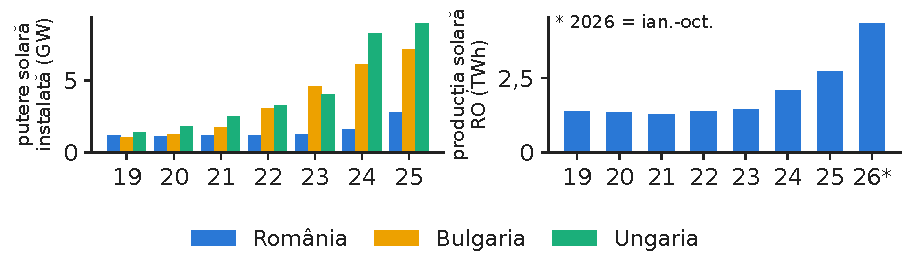
\includegraphics[width=\textwidth,height=0.477\textheight,keepaspectratio]{charts/ro/solar_growth.pdf}\end{center}\vspace{-3mm}
\chartsource{Sursa: energy-charts.info (Fraunhofer ISE), puterea instalată din ENTSO-E; producția solară, ENTSO-E (date Transelectrica). Date: puterea instalată la sfîrșitul anilor 2019-2025; producția 2019 - 2026-10-31.}
\vspace{0.5mm}
\begin{itemize}\setlength{\itemsep}{0pt}
  \item \textbf{Producția solară a României, ianuarie--octombrie}: 2{,}53 TWh în 2025 și 4{,}32 TWh în 2026
    \begin{itemize}\setlength{\itemsep}{0pt}
      \item 2{,}3\% din consum în 2019, 10{,}2\% în 2026; vecinii: Bulgaria 7{,}2 GW, Ungaria 9{,}0 GW
    \end{itemize}
\end{itemize}
\par\vfill\manager{un parc solar nou vinde în aceleași ore însorite ca toate parcurile existente, din România și din țările vecine.}\par\vspace{0.5mm}
\par\vfill\noindent{\scriptsize\color{FooterGray}(ENTSO-E; producția măsurată poate omite panourile de pe acoperișuri)}\hfill\qlink{EMQA\_L6\_solar\_growth}{Quantlets/L6/EMQA_L6_solar_growth}\par\vspace{0.5mm}
\end{frame}

\subsection{Efectul ordinii de merit}

\begin{frame}{Oferta cu cost zero deplasează curba ofertei spre dreapta și reduce prețul de închidere}
\footnotesize
\intuition{Solarul și eolianul ofertează aproape de zero; ofertele mai scumpe se mută spre dreapta, iar intersecția cu cererea coboară.}
\begin{columns}[T,onlytextwidth]
\begin{column}{0.50\textwidth}
\[ S(p)+X\cdot\mathbf 1[p\ge 0]=D(p)\ \Rightarrow\ p^*(X) \]\vspace{-2mm}\[ \frac{\mathrm dp^*}{\mathrm dX}=-\frac{1}{S'(p^*)-D'(p^*)} \]{\footnotesize\begin{itemize}\setlength{\itemsep}{0pt}
  \item \textbf{\txtwhere}
    \begin{itemize}\setlength{\itemsep}{0pt}
      \item $S(p)$ = MW oferiți la prețuri $\le p$
      \item $D(p)$ = MW ceruți la prețuri $\ge p$
      \item $X$ = MW în plus, oferiți la 0 EUR/MWh
      \item $S'$, $D'$ = pantele curbelor (MW pentru 1 EUR/MWh).
    \end{itemize}
\end{itemize}\par}
\end{column}
\begin{column}{0.47\textwidth}
\begin{itemize}\setlength{\itemsep}{2pt}
  \item \textbf{Cum se citește formula}
    \begin{itemize}\setlength{\itemsep}{0pt}
      \item Curbe plate în jurul prețului: efect mic
      \item Curbe abrupte: efect mare
    \end{itemize}
  \item \textbf{OPCOM, 21 octombrie 2026, 12:00--12:15}
    \begin{itemize}\setlength{\itemsep}{0pt}
      \item Prețul: 152{,}23 EUR/MWh
      \item Doar 34 MW oferiți între 1 EUR/MWh și acest preț
    \end{itemize}
\end{itemize}
\end{column}
\end{columns}
\par\vfill\manager{cu cît curba locală este mai abruptă, cu atît un parc nou își modifică mai mult propriul preț.}\par\vspace{0.5mm}
\par\vfill\noindent{\scriptsize\color{FooterGray}(Sensfuß, Ragwitz \& Genoese, 2008, ENPOL)}\hfill\tryit{notebook-ul Jupyter, secțiunea 2}\par\vspace{0.5mm}
\end{frame}

\begin{frame}{Ofertele din România: +40 MW la preț zero coboară amiaza sub 50 EUR/MWh}
\footnotesize
\begin{center}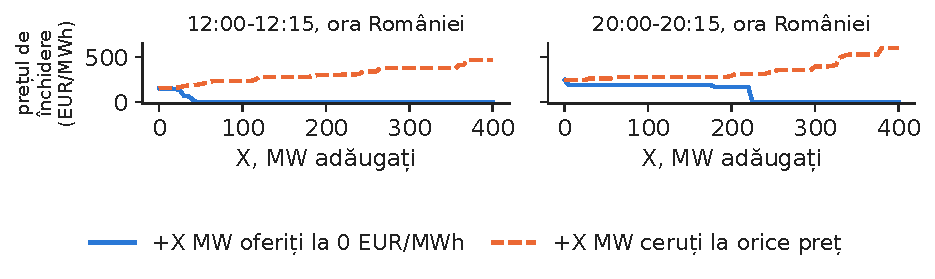
\includegraphics[width=\textwidth,height=0.451\textheight,keepaspectratio]{charts/ro/merit_shift.pdf}\end{center}\vspace{-3mm}
\chartsource{Sursa: OPCOM, curbele agregate PZU (XML), calcule proprii. Date: ziua de livrare 2026-10-21; fluxurile transfrontaliere, blocurile și ordinele orare rămîn la valorile acceptate.}
\vspace{0.5mm}
\begin{itemize}\setlength{\itemsep}{0pt}
  \item \textbf{La amiază}: +25 MW la preț zero, 152{,}23 $\to$ 131{,}40 EUR/MWh
    \begin{itemize}\setlength{\itemsep}{0pt}
      \item Seara: importul net de 1\,054 MW adîncește curba; pentru aceeași scădere sînt necesari 225 MW
      \item Fluxurile rămîn fixe, deci rezultatul este o limită superioară pentru piața cuplată
    \end{itemize}
\end{itemize}
\par\vfill\manager{pentru Transelectrica: interconexiunile, nu centralele locale, dau profunzime prețului de la amiază.}\par\vspace{0.5mm}
\par\vfill\noindent{\scriptsize\color{FooterGray}(curbele agregate OPCOM; calcule proprii)}\hfill\qlink{EMQA\_L6\_merit\_shift}{Quantlets/L6/EMQA_L6_merit_shift}\par\vspace{0.5mm}
\end{frame}

\begin{frame}{În piața cuplată, 1 GW solar în plus reduce prețul din România cu aproximativ 27 EUR/MWh}
\footnotesize
\intuition{La aceeași oră și în aceeași lună, orele cu mai mult soare și vînt sînt mai ieftine.}
\begin{columns}[T,onlytextwidth]
\begin{column}{0.49\textwidth}
\[ P_t=\underbrace{\alpha_{m(t)}+\gamma_{h(t)}+\delta_{w(t)}}_{\text{efecte fixe}}+\beta_L L_t+\beta_W W_t+\beta_S S_t+\varepsilon_t \]{\footnotesize\begin{itemize}\setlength{\itemsep}{0pt}
  \item \textbf{\txtwhere}
    \begin{itemize}\setlength{\itemsep}{0pt}
      \item $P_t$ = prețul orar (EUR/MWh), $L_t$, $W_t$, $S_t$ = consumul, producția eoliană și cea solară (GW)
      \item $\alpha$, $\gamma$, $\delta$ = constante pentru lună (gaze, carbon), oră și ziua săptămînii, estimate prin metoda celor mai mici pătrate (OLS).
    \end{itemize}
\end{itemize}\par}
\end{column}
\begin{column}{0.48\textwidth}
\begin{itemize}\setlength{\itemsep}{2pt}
  \item \textbf{Estimări}, 33\,600 de ore, 2023 -- octombrie 2026, $R^2$ = 0{,}65
    \begin{itemize}\setlength{\itemsep}{0pt}
      \item EUR/MWh pentru 1 GW: solar \ensuremath{-}26{,}7, eolian \ensuremath{-}15{,}3, consum \ensuremath{+}40{,}7
      \item Eroarea standard (SE) pentru solar: 2{,}2, robustă la heteroscedasticitate și autocorelare (HAC)
    \end{itemize}
  \item \textbf{La amiază, în 2026}
    \begin{itemize}\setlength{\itemsep}{0pt}
      \item 1{,}62 GW solar în medie: \ensuremath{-}43{,}3 EUR/MWh; o asociere, nu un efect cauzal
    \end{itemize}
\end{itemize}
\end{column}
\end{columns}
\par\vfill\manager{un furnizor care cumpără blocuri de amiază le plătește mai puțin în zilele însorite, cu aproximativ această sumă.}\par\vspace{0.5mm}
\par\vfill\noindent{\scriptsize\color{FooterGray}(Cludius et al., 2014, ENEECO; Würzburg et al., 2013, ENEECO)}\hfill\tryit{notebook-ul Jupyter, secțiunea 3}\par\vspace{0.5mm}
\end{frame}

\begin{frame}{Prețul crește cu consumul rezidual; orele sub 2 GW au ajuns la 9{,}0\% în 2026}
\footnotesize
\begin{center}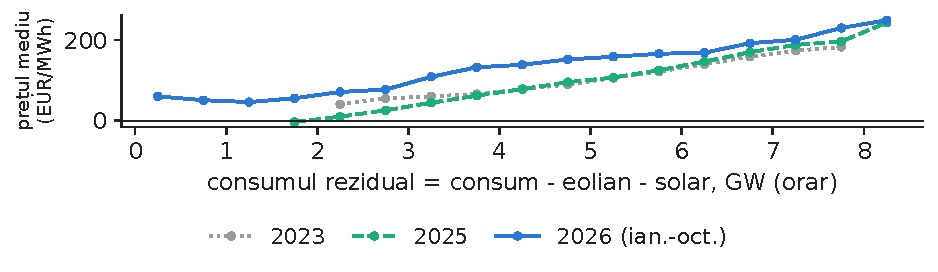
\includegraphics[width=\textwidth,height=0.435\textheight,keepaspectratio]{charts/ro/resid_price.pdf}\end{center}\vspace{-3mm}
\chartsource{Sursa: energy-charts.info (Fraunhofer ISE); prețuri OPCOM; producția solară și eoliană și consumul, ENTSO-E (date Transelectrica). Date: orar, 2023-01-01 - 2026-10-31; intervale de 0,5 GW cu cel puțin 20 de ore.}
\vspace{0.5mm}
\begin{itemize}\setlength{\itemsep}{0pt}
  \item \textbf{Consumul rezidual} = consum $-$ eolian $-$ solar, adică cererea rămasă pentru celelalte centrale și pentru import
    \begin{itemize}\setlength{\itemsep}{0pt}
      \item +1 GW crește prețul cu 28{,}3 EUR/MWh (SE 0{,}9), cu aceleași efecte fixe
      \item Orele sub 2 GW: 0{,}1\% în 2023, 9{,}0\% în 2026
    \end{itemize}
\end{itemize}
\par\vfill\manager{un producător hidro păstrează apa pentru orele cu consum rezidual mare, cînd fiecare GW valorează cel mai mult.}\par\vspace{0.5mm}
\par\vfill\noindent{\scriptsize\color{FooterGray}(calcule proprii)}\hfill\qlink{EMQA\_L6\_resid\_price}{Quantlets/L6/EMQA_L6_resid_price}\par\vspace{0.5mm}
\end{frame}

\subsection{Sursele regenerabile și rețeaua: redispecerizarea}

\begin{frame}{Cercetarea grupului nostru: învățarea automată prognozează redispecerizarea din Germania cu o zi înainte}
\footnotesize
\begin{itemize}\setlength{\itemsep}{2pt}
  \item \textbf{De ce redispecerizare}: vîntul este în nordul Germaniei, consumul în sudul industrializat
    \begin{itemize}\setlength{\itemsep}{0pt}
      \item După piața pentru ziua următoare, operatorii de transport și de sistem cer centralelor să crească sau să reducă producția
    \end{itemize}
  \item \textbf{Ce a făcut lucrarea}: a prognozat volumul orar al redispecerizării (MW), în sus și în jos, la cei patru operatori germani
    \begin{itemize}\setlength{\itemsep}{0pt}
      \item Cu 24 h înainte, cu ce se știe în după-amiaza zilei $d-1$: vînt, solar, consum, diferențe de preț, schimburi programate
      \item Date oct.\ 2021 -- feb.\ 2026; 11 ferestre lunare de test, mar.\ 2025 -- feb.\ 2026
    \end{itemize}
  \item \textbf{Ce a găsit}: rețelele neuronale adînci sînt cel mai des printre cele mai bune modele
    \begin{itemize}\setlength{\itemsep}{0pt}
      \item Cea mai bună dintre ele intră în mulțimea de încredere a modelelor (eroarea absolută medie) pentru 6 din cele 8 serii
      \item Variabilele explicative ajută doar aliniate în timp: prognoze semnificativ mai bune în 40--60\% dintre seriile dense
    \end{itemize}
\end{itemize}
\par\vfill\manager{pentru Transelectrica: prognozați cu o zi înainte unde vor atinge eolianul și solarul limitele rețelei.}\par\vspace{0.5mm}
\par\vfill\noindent{\scriptsize\color{FooterGray}(Basangova, Bolovăneanu, Conda, Erlwein-Sayer, Melzer, Pele, Petukhina \& Phan, 2026, prezentare la AIDA 2026 (AI and Digital Assets in Energy and Finance), București, 3 iunie 2026: \href{https://github.com/danpele/EMQA/blob/main/resources/aida2026/bolovaneanu_redispatch_forecasting.pdf}{diapozitive})}\par\vspace{0.5mm}
\end{frame}


\section{Prețul capturat și canibalizarea}

\subsection{Definiții}

\begin{frame}{Prețul capturat este prețul mediu ponderat cu producția centralei}
\footnotesize
\intuition{Un parc solar încasează prețul intervalelor în care produce, nu media tuturor intervalelor.}
\begin{columns}[T,onlytextwidth]
\begin{column}{0.50\textwidth}
\[ \mathrm{CP}=\frac{\sum_t P_t G_t\Delta_t}{\sum_t G_t\Delta_t},\qquad B=\frac{\sum_t P_t\Delta_t}{\sum_t\Delta_t} \]\[ \mathrm{CR}=\frac{\mathrm{CP}}{B}=1+\frac{\mathrm{Cov}_\Delta(P,G)}{\bar P\,\bar G} \]{\footnotesize\begin{itemize}\setlength{\itemsep}{0pt}
  \item \textbf{\txtwhere}
    \begin{itemize}\setlength{\itemsep}{0pt}
      \item Prețul capturat (CP), prețul de bază $B$, rata de captare (CR)
      \item $P_t$ = prețul, $G_t$ = producția (MW), $\Delta_t$ = 1 h sau 0{,}25 h, $\mathrm{Cov}_\Delta$ = covarianța ponderată cu durata (Anexa A).
    \end{itemize}
\end{itemize}\par}
\end{column}
\begin{column}{0.47\textwidth}
\begin{itemize}\setlength{\itemsep}{2pt}
  \item \textbf{Solarul din România, ian.--oct. 2026}
    \begin{itemize}\setlength{\itemsep}{0pt}
      \item CP 85{,}0, $B$ 137{,}5 EUR/MWh; CR 61{,}9\%
      \item Corelația dintre preț și producție: \ensuremath{-}0{,}43; de aceea CR este sub 1
    \end{itemize}
  \item \textbf{Eolianul din România, aceeași perioadă}
    \begin{itemize}\setlength{\itemsep}{0pt}
      \item CR 103{,}0\%; vîntul bate și noaptea, și iarna
    \end{itemize}
\end{itemize}
\end{column}
\end{columns}
\par\vfill\manager{prețul unui contract pe termen lung pentru energie solară (PPA) pornește de la prețul capturat, nu de la prețul de bază.}\par\vspace{0.5mm}
\par\vfill\noindent{\scriptsize\color{FooterGray}(Hirth, 2013, ENEECO; Hirth, Ueckerdt \& Edenhofer, 2016, Energy J.)}\hfill\tryit{notebook-ul Jupyter, secțiunea 4}\par\vspace{0.5mm}
\end{frame}

\subsection{România, an de an}

\begin{frame}{Rata de captare a solarului în România a scăzut de la 104\% în 2019 la 59\% în 2025}
\footnotesize
\begin{center}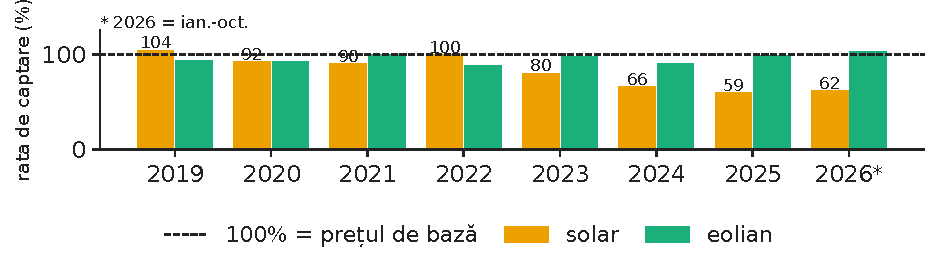
\includegraphics[width=\textwidth,height=0.407\textheight,keepaspectratio]{charts/ro/capture_rates.pdf}\end{center}\vspace{-3mm}
\chartsource{Sursa: energy-charts.info (Fraunhofer ISE); prețuri OPCOM; producția solară și eoliană și consumul, ENTSO-E (date Transelectrica). Date: 2019 - 2026-10-31; date orare pînă în sep. 2025, la 15 minute din oct. 2025.}
\vspace{0.5mm}
\begin{itemize}\setlength{\itemsep}{0pt}
  \item \textbf{Solarul}: scăderea începe în 2023, odată cu creșterea producției
    \begin{itemize}\setlength{\itemsep}{0pt}
      \item 2026: 61{,}9\%, deși producția a crescut cu 71\% față de aceleași luni din 2025
      \item Eolianul: între 88\% și 103\%, fără tendință, deoarece producția eoliană nu a crescut
    \end{itemize}
\end{itemize}
\par\vfill\manager{o bancă ce finanțează un proiect solar trebuie să înmulțească prețul de bază cu rata de captare.}\par\vspace{0.5mm}
\par\vfill\noindent{\scriptsize\color{FooterGray}(calcule proprii)}\hfill\qlink{EMQA\_L6\_capture\_rates}{Quantlets/L6/EMQA_L6_capture_rates}\par\vspace{0.5mm}
\end{frame}

\begin{frame}{În 2025, un MWh solar din România a obținut cu 43{,}9 EUR mai puțin decît prețul de bază}
\footnotesize
\begin{center}{\footnotesize\renewcommand{\arraystretch}{1.05}\setlength{\tabcolsep}{4pt}
\begin{tabular}{@{}lrrrrrrrr@{}}\toprule
Anul & $B$ & CP solar & CR solar, \% & $B-\mathrm{CP}$ & CP eolian & CR eolian, \% & TWh solar & TWh eolian \\ \midrule
2019 & 50{,}4 & 52{,}7 & \cellcolor{Forest!54}104{,}5 & \ensuremath{-}2{,}3 & 47{,}2 & \cellcolor{Forest!30}93{,}6 & 1{,}37 & 6{,}68 \\
2020 & 39{,}5 & 36{,}4 & \cellcolor{Forest!27}92{,}2 & \ensuremath{+}3{,}1 & 36{,}6 & \cellcolor{Forest!28}92{,}6 & 1{,}34 & 6{,}89 \\
2021 & 111{,}4 & 100{,}6 & \cellcolor{Forest!23}90{,}3 & \ensuremath{+}10{,}8 & 111{,}0 & \cellcolor{Forest!43}99{,}6 & 1{,}29 & 6{,}44 \\
2022 & 265{,}3 & 264{,}0 & \cellcolor{Forest!43}99{,}5 & \ensuremath{+}1{,}3 & 234{,}4 & \cellcolor{Forest!18}88{,}4 & 1{,}37 & 6{,}92 \\
2023 & 103{,}7 & 83{,}2 & 80{,}2 & \ensuremath{+}20{,}6 & 101{,}0 & \cellcolor{Forest!38}97{,}4 & 1{,}46 & 7{,}45 \\
2024 & 103{,}5 & 68{,}0 & \cellcolor{Crimson!31}65{,}7 & \ensuremath{+}35{,}5 & 93{,}4 & \cellcolor{Forest!22}90{,}2 & 2{,}09 & 6{,}34 \\
2025 & 108{,}2 & 64{,}2 & \cellcolor{Crimson!45}59{,}4 & \ensuremath{+}43{,}9 & 106{,}7 & \cellcolor{Forest!41}98{,}7 & 2{,}72 & 5{,}88 \\
2026* & 137{,}5 & 85{,}0 & \cellcolor{Crimson!40}61{,}9 & \ensuremath{+}52{,}4 & 141{,}6 & \cellcolor{Forest!51}103{,}0 & 4{,}32 & 5{,}27 \\
\bottomrule\end{tabular}}\end{center}\vspace{-2mm}\begin{itemize}\setlength{\itemsep}{1pt}
  \item \textbf{Cum se citește tabelul}: $B$ și CP în EUR/MWh; verde = CR aproape de 100\%, roșu = mult sub
    \begin{itemize}\setlength{\itemsep}{0pt}
      \item * 2026 = ian.--oct. 2026; 2022 = criza energetică, toate prețurile au fost mari
    \end{itemize}
\end{itemize}
\par\vfill\manager{diferența $B-\mathrm{CP}$ este un cost suportat de dezvoltatorul solar
    \begin{itemize}\setlength{\itemsep}{0pt}
      \item A crescut în fiecare an din 2022.
    \end{itemize}}\par\vspace{0.5mm}
\par\vfill\noindent{\scriptsize\color{FooterGray}(calcule proprii)}\hfill\tryit{notebook-ul Jupyter, secțiunea 4}\par\vspace{0.5mm}
\end{frame}

\subsection{Canibalizarea}

\begin{frame}{Cînd ponderea solarului în consumul lunii crește cu un punct procentual, rata de captare solară scade cu circa 4{,}2 puncte}
\footnotesize
\begin{center}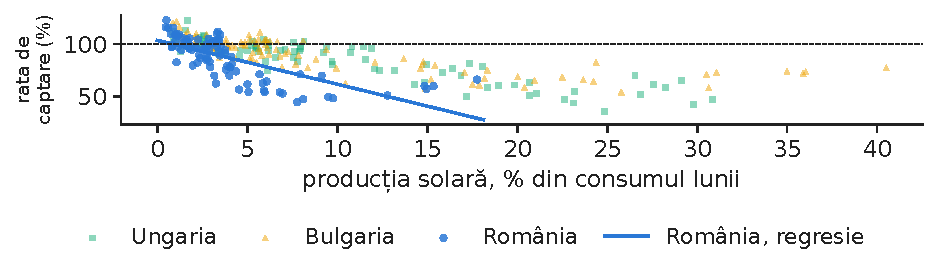
\includegraphics[width=\textwidth,height=0.415\textheight,keepaspectratio]{charts/ro/cannibal.pdf}\end{center}\vspace{-3mm}
\chartsource{Sursa: energy-charts.info (Fraunhofer ISE); prețuri pentru ziua următoare (OPCOM, IBEX, HUPX); producția solară și consumul, ENTSO-E. Date: lunar, 2019-01 - 2026-10; Ungaria din oct. 2019.}
\vspace{0.5mm}
\begin{itemize}\setlength{\itemsep}{0pt}
  \item \textbf{Regresia} $\mathrm{CR}_m=a+b\,s_m+u_m$, unde $s_m$ = producția solară, în \% din consumul lunii $m$
    \begin{itemize}\setlength{\itemsep}{0pt}
      \item România: $\hat b$ = \ensuremath{-}4{,}20 (SE 1{,}03), $R^2$ = 0{,}53, 94 de luni
      \item Ungaria \ensuremath{-}2{,}14, Bulgaria \ensuremath{-}1{,}32; prețul din România scade și cu producția solară a vecinilor
    \end{itemize}
\end{itemize}
\par\vfill\manager{pentru venitul unui parc, prognozați producția solară regională, nu doar pe cea a României.}\par\vspace{0.5mm}
\par\vfill\noindent{\scriptsize\color{FooterGray}(López Prol, Steininger \& Zilberman, 2020, ENEECO)}\hfill\qlink{EMQA\_L6\_cannibal}{Quantlets/L6/EMQA_L6_cannibal}\par\vspace{0.5mm}
\end{frame}

\begin{frame}{Rata de captare solară a scăzut simultan în România, Bulgaria și Ungaria}
\footnotesize
\begin{center}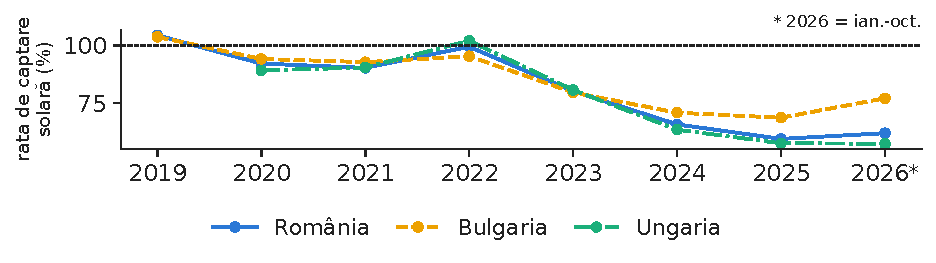
\includegraphics[width=\textwidth,height=0.517\textheight,keepaspectratio]{charts/ro/capture_region.pdf}\end{center}\vspace{-3mm}
\chartsource{Sursa: energy-charts.info (Fraunhofer ISE); prețuri pentru ziua următoare (OPCOM, IBEX, HUPX); producția solară și consumul, ENTSO-E. Date: 2019 (Ungaria 2020) - 2026-10-31; Bulgaria: producție solară orară.}
\vspace{0.5mm}
\begin{itemize}\setlength{\itemsep}{0pt}
  \item \textbf{2025}: România 59{,}4\%, Bulgaria 68{,}6\%, Ungaria 57{,}5\%
    \begin{itemize}\setlength{\itemsep}{0pt}
      \item 2026: Bulgaria urcă la 77{,}1\%, odată cu extinderea bateriilor; este o asociere, nu o dovadă
    \end{itemize}
\end{itemize}
\par\vfill\manager{un parc solar cîștigă și din bateriile altora, care se încarcă la amiază și îi cresc prețul.}\par\vspace{0.5mm}
\par\vfill\noindent{\scriptsize\color{FooterGray}(calcule proprii; producția din Bulgaria este orară)}\hfill\qlink{EMQA\_L6\_capture\_region}{Quantlets/L6/EMQA_L6_capture_region}\par\vspace{0.5mm}
\end{frame}

\begin{frame}{În 2025, 32{,}1\% din energia solară s-a vîndut în cele mai ieftine 10\% dintre ore}
\footnotesize
\begin{center}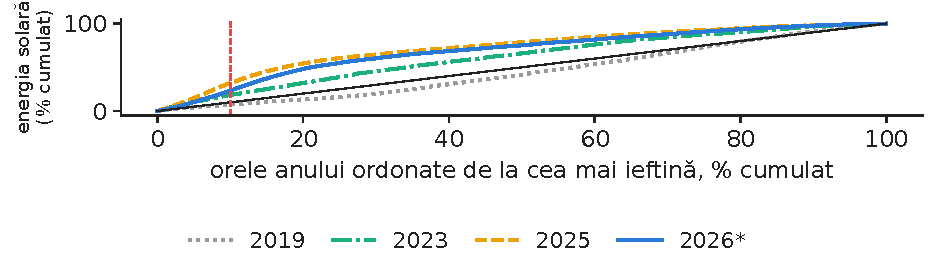
\includegraphics[width=\textwidth,height=0.458\textheight,keepaspectratio]{charts/ro/cheap_hours.pdf}\end{center}\vspace{-3mm}
\chartsource{Sursa: energy-charts.info (Fraunhofer ISE); prețuri OPCOM; producția solară și eoliană și consumul, ENTSO-E (date Transelectrica). Date: fiecare an calendaristic; 2026 pînă la 2026-10-31.}
\vspace{0.5mm}
\begin{itemize}\setlength{\itemsep}{0pt}
  \item \textbf{Citire}: orele sînt ordonate de la cea mai ieftină; curba = partea din energia solară a anului produsă pînă la acel rang
    \begin{itemize}\setlength{\itemsep}{0pt}
      \item 2019: 7{,}6\%; 2025: 32{,}1\%; 2026: 23{,}4\%; la prețuri nule sau negative: 9{,}6\% din producția anului 2025
    \end{itemize}
\end{itemize}
\par\vfill\manager{cum am anunțat în cursul 1: un parc solar fără stocare vinde mult în cele mai ieftine ore ale anului.}\par\vspace{0.5mm}
\par\vfill\noindent{\scriptsize\color{FooterGray}(calcule proprii)}\hfill\qlink{EMQA\_L6\_cheap\_hours}{Quantlets/L6/EMQA_L6_cheap_hours}\par\vspace{0.5mm}
\end{frame}


\section{Prețurile negative}

\begin{frame}{Un producător ofertează sub zero cînd oprirea îl costă mai mult decît plata pentru a produce}
\footnotesize
\intuition{Oferta este costul unui MWh în plus, minus ce primește sau economisește centrala doar dacă funcționează.}
\begin{columns}[T,onlytextwidth]
\begin{column}{0.44\textwidth}
\[ b_i=c_i-s_i-k_i,\qquad h^{-}=\textstyle\sum_t \Delta_t\,\mathbf 1[P_t<0] \]{\footnotesize\begin{itemize}\setlength{\itemsep}{0pt}
  \item \textbf{\txtwhere}
    \begin{itemize}\setlength{\itemsep}{0pt}
      \item $b_i$ = oferta centralei $i$ (EUR/MWh), $c_i$ = costul marginal
      \item $s_i$ = sprijinul plătit pe MWh produs, $k_i$ = costul repornirii, pe MWh al unei opriri
      \item $h^-$ = orele cu preț negativ, în ore echivalente.
    \end{itemize}
\end{itemize}\par}
\end{column}
\begin{column}{0.53\textwidth}
\begin{itemize}\setlength{\itemsep}{2pt}
  \item \textbf{Cine ofertează sub zero}
    \begin{itemize}\setlength{\itemsep}{0pt}
      \item Producția plătită pe MWh printr-o schemă de sprijin sau un contract
      \item Centralele nucleare și hidro pe firul apei, care nu se pot opri ieftin
    \end{itemize}
  \item \textbf{România, 2025}
    \begin{itemize}\setlength{\itemsep}{0pt}
      \item 196 de ore negative; prețul negativ mediu: \ensuremath{-}10{,}5 EUR/MWh
      \item Cel mai mic preț din 2026: \ensuremath{-}99{,}75 EUR/MWh
    \end{itemize}
\end{itemize}
\end{column}
\end{columns}
\par\vfill\manager{un parc solar fără sprijin are $b_i\approx 0$, deci trebuie să se oprească imediat ce prețul devine negativ.}\par\vspace{0.5mm}
\par\vfill\noindent{\scriptsize\color{FooterGray}(Fanone, Gamba \& Prokopczuk, 2013, ENEECO)}\hfill\tryit{notebook-ul Jupyter, secțiunea 5}\par\vspace{0.5mm}
\end{frame}

\begin{frame}{România a avut 196 de ore cu preț negativ în 2025, Germania 575}
\footnotesize
\begin{center}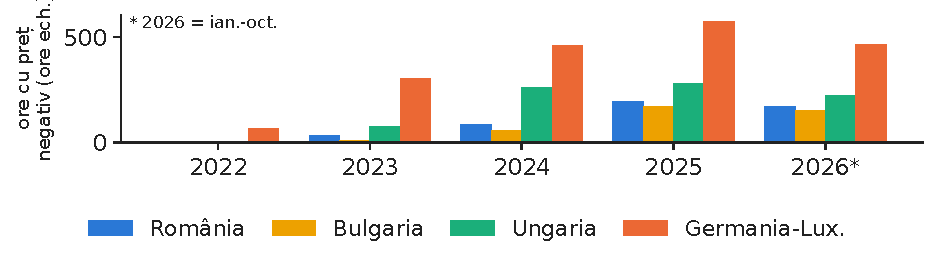
\includegraphics[width=\textwidth,height=0.479\textheight,keepaspectratio]{charts/ro/neg_hours.pdf}\end{center}\vspace{-3mm}
\chartsource{Sursa: energy-charts.info (Fraunhofer ISE); prețurile pieței pentru ziua următoare: OPCOM (RO), IBEX (BG), HUPX (HU), EPEX SPOT (DE-LU), prin ENTSO-E. Date: 2022 - 2026-10-31; un interval de 15 minute contează 0,25 h.}
\vspace{0.5mm}
\begin{itemize}\setlength{\itemsep}{0pt}
  \item \textbf{Ianuarie--octombrie, 2025 față de 2026}: România 196 $\to$ 171{,}75 h, Ungaria 281 $\to$ 223{,}5 h
    \begin{itemize}\setlength{\itemsep}{0pt}
      \item Mai puține, deși solarul a crescut; explicații posibile: prețuri mai mari în general, mai multe baterii care se încarcă la amiază
    \end{itemize}
\end{itemize}
\par\vfill\manager{un furnizor cu clienți industriali flexibili poate fi plătit pentru a consuma în aceste ore.}\par\vspace{0.5mm}
\par\vfill\noindent{\scriptsize\color{FooterGray}(calcule proprii; regula de numărare din cursul 1)}\hfill\qlink{EMQA\_L6\_neg\_hours}{Quantlets/L6/EMQA_L6_neg_hours}\par\vspace{0.5mm}
\end{frame}

\begin{frame}{Oprirea la prețuri negative aduce puțin; pierderea reală vine din prețul mic, dar pozitiv, de la amiază}
\footnotesize
\intuition{Un parc fără sprijin cîștigă $|P_t|$ pentru fiecare MWh neprodus la preț negativ; acești MWh sînt puțini.}
\begin{columns}[T,onlytextwidth]
\begin{column}{0.50\textwidth}
\[ g=\frac{\sum_t \max(0,-P_t)\,G_t\Delta_t}{\sum_t G_t\Delta_t}\quad\text{față de}\quad B-\mathrm{CP} \]{\footnotesize\begin{itemize}\setlength{\itemsep}{0pt}
  \item \textbf{\txtwhere}
    \begin{itemize}\setlength{\itemsep}{0pt}
      \item $G_t$ = producția solară (MW)
      \item $g$ = cîștigul pe MWh de producție anuală, dacă parcul se oprește în toate intervalele negative
      \item $B-\mathrm{CP}$ = reducerea datorată profilului.
    \end{itemize}
\end{itemize}\par}
\end{column}
\begin{column}{0.47\textwidth}
\begin{itemize}\setlength{\itemsep}{2pt}
  \item \textbf{Solarul din România, 2025}
    \begin{itemize}\setlength{\itemsep}{0pt}
      \item 6{,}2\% din producție la prețuri negative, cu un cost de 1{,}71 milioane EUR
      \item $g$ = 0{,}63, față de $B-\mathrm{CP}$ = 43{,}9 EUR/MWh
    \end{itemize}
  \item \textbf{2026}
    \begin{itemize}\setlength{\itemsep}{0pt}
      \item 4{,}0\% din producție; $g$ = 0{,}35 EUR/MWh
    \end{itemize}
\end{itemize}
\end{column}
\end{columns}
\par\vfill\manager{instalați oprirea la distanță, pentru că este ieftină, dar evaluați parcul după prețul capturat.}\par\vspace{0.5mm}
\par\vfill\noindent{\scriptsize\color{FooterGray}(calcule proprii)}\hfill\tryit{notebook-ul Jupyter, secțiunea 5}\par\vspace{0.5mm}
\end{frame}

\begin{frame}{Sferturile de oră arată 26 prețuri negative ascunse în ore cu medie nenegativă}
\footnotesize
\begin{itemize}\setlength{\itemsep}{4pt}
  \item \textbf{De la 1 octombrie 2025}, cînd cuplarea unică a piețelor pentru ziua următoare (SDAC) a trecut la MTU de 15 minute
    \begin{itemize}\setlength{\itemsep}{0pt}
      \item 687 de sferturi de oră negative în România = 171{,}75 ore echivalente
      \item 26 de dintre ele (3{,}8\%) sînt în ore cu media zero sau pozitivă
    \end{itemize}
  \item \textbf{De ce contează}
    \begin{itemize}\setlength{\itemsep}{0pt}
      \item Mediile orare arată doar 195 de ore negative
      \item O baterie sau un consumator flexibil care acționează pe sfert de oră le poate valorifica; un parc măsurat pe sfert de oră le plătește
    \end{itemize}
  \item \textbf{Regula de numărare}
    \begin{itemize}\setlength{\itemsep}{0pt}
      \item $h^-=\sum_t\Delta_t\mathbf 1[P_t<0]$, $\Delta_t$ = 0{,}25 h; un sfert de oră nu se numără niciodată ca o oră
    \end{itemize}
\end{itemize}
\par\vfill\manager{programați oprirea centralelor și bateriile pe intervale de 15 minute, ca piața.}\par\vspace{0.5mm}
\par\vfill\noindent{\scriptsize\color{FooterGray}(NEMO Committee, 2025; calcule proprii)}\hfill\tryit{notebook-ul Jupyter, secțiunea 5}\par\vspace{0.5mm}
\end{frame}


\section{Profilul zilnic și diferențele de preț}

\begin{frame}{Primăvara, prețul mediu: 23{,}0 EUR/MWh la amiază, 208{,}3 seara}
\footnotesize
\begin{center}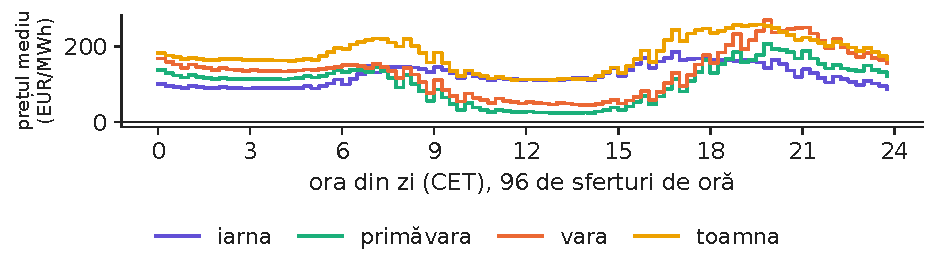
\includegraphics[width=\textwidth,height=0.491\textheight,keepaspectratio]{charts/ro/shape15.pdf}\end{center}\vspace{-3mm}
\chartsource{Sursa: energy-charts.info (Fraunhofer ISE); prețurile PZU ale OPCOM pentru România, prin ENTSO-E. Date: ultimele 12 luni, 2025-11-01 - 2026-10-31, prețuri pe 15 minute, ora CET; iarna = dec.-feb., primăvara = mar.-mai, vara = iun.-aug., toamna = sep.-nov..}
\vspace{0.5mm}
\begin{itemize}\setlength{\itemsep}{0pt}
  \item \textbf{„Valea” solară}: primăvara, minimul este la 12:45, iar maximul la 19:45 CET
    \begin{itemize}\setlength{\itemsep}{0pt}
      \item Maximul minus minimul: primăvara 185, vara 226, iarna doar 98 EUR/MWh
    \end{itemize}
\end{itemize}
\par\vfill\manager{o baterie se încarcă în „vale” și se descarcă seara: diferența este marja ei brută.}\par\vspace{0.5mm}
\par\vfill\noindent{\scriptsize\color{FooterGray}(calcule proprii, ultimele 12 luni (noiembrie 2025 -- octombrie 2026))}\hfill\qlink{EMQA\_L6\_shape15}{Quantlets/L6/EMQA_L6_shape15}\par\vspace{0.5mm}
\end{frame}

\begin{frame}{O baterie cîștigă diferența dintre orele scumpe și cele ieftine, mai puțin pierderile}
\footnotesize
\intuition{Bateria cumpără un MWh cînd este ieftin și vinde, cînd este scump, ce rămîne după încărcare și descărcare.}
\begin{columns}[T,onlytextwidth]
\begin{column}{0.50\textwidth}
\[ S^{(k)}_d=\bar P^{\,\mathrm{top}\,k}_d-\bar P^{\,\mathrm{bot}\,k}_d \]\[ \pi_d\approx k\,\big(\eta\,\bar P^{\,\mathrm{top}\,k}_d-\bar P^{\,\mathrm{bot}\,k}_d\big) \]{\footnotesize\begin{itemize}\setlength{\itemsep}{0pt}
  \item \textbf{\txtwhere}
    \begin{itemize}\setlength{\itemsep}{0pt}
      \item $\bar P^{\,\mathrm{top}\,k}_d$, $\bar P^{\,\mathrm{bot}\,k}_d$ = prețul mediu al celor mai scumpe, respectiv al celor mai ieftine $k$ ore din ziua $d$
      \item $k$ = orele de stocare
      \item $\eta$ = randamentul ciclului complet (85\%), $\pi_d$ = marja brută a unui ciclu, 1 MW (EUR).
    \end{itemize}
\end{itemize}\par}
\end{column}
\begin{column}{0.47\textwidth}
\begin{itemize}\setlength{\itemsep}{2pt}
  \item \textbf{România, $k=2$, diferența zilnică medie}
    \begin{itemize}\setlength{\itemsep}{0pt}
      \item 45 EUR/MWh în 2019, 151 în 2025, 174 în 2026
    \end{itemize}
  \item \textbf{Pierderile impun un prag}
    \begin{itemize}\setlength{\itemsep}{0pt}
      \item Dacă bateria cumpără la 50 EUR/MWh, trebuie să vîndă peste $50/0{,}85\approx59$ EUR/MWh
    \end{itemize}
\end{itemize}
\end{column}
\end{columns}
\par\vfill\manager{un dezvoltator de baterii citește cazul de afaceri din diferența zilnică de preț, înaintea oricărui model.}\par\vspace{0.5mm}
\par\vfill\noindent{\scriptsize\color{FooterGray}(Sioshansi et al., 2009, ENEECO)}\hfill\tryit{notebook-ul Jupyter, secțiunea 6}\par\vspace{0.5mm}
\end{frame}

\begin{frame}{Diferența zilnică de preț este de circa patru ori mai mare decît în 2019 și asemănătoare în România, Bulgaria și Ungaria}
\footnotesize
\begin{center}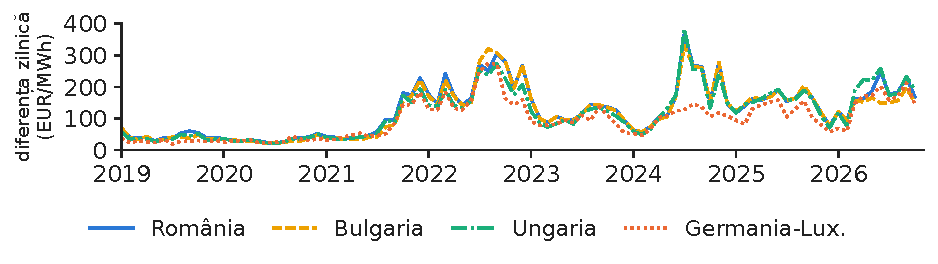
\includegraphics[width=\textwidth,height=0.405\textheight,keepaspectratio]{charts/ro/spreads.pdf}\end{center}\vspace{-3mm}
\chartsource{Sursa: energy-charts.info (Fraunhofer ISE); prețurile pieței pentru ziua următoare: OPCOM (RO), IBEX (BG), HUPX (HU), EPEX SPOT (DE-LU), prin ENTSO-E. Date: zilnic, prețuri orare (media sferturilor), medii lunare, 2019 - 2026-10-31.}
\vspace{0.5mm}
\begin{itemize}\setlength{\itemsep}{0pt}
  \item \textbf{Cele mai scumpe 2 ore minus cele mai ieftine 2 ore, 2026}: România 174, Bulgaria 150, Ungaria 187, Germania 152 EUR/MWh
    \begin{itemize}\setlength{\itemsep}{0pt}
      \item Piețele sînt cuplate, deci toate bateriile din regiune concurează pentru aceeași diferență
    \end{itemize}
\end{itemize}
\par\vfill\manager{tratați diferența de preț ca pe o resursă regională, împărțită cu fiecare baterie nouă din țările vecine.}\par\vspace{0.5mm}
\par\vfill\noindent{\scriptsize\color{FooterGray}(calcule proprii)}\hfill\qlink{EMQA\_L6\_spreads}{Quantlets/L6/EMQA_L6_spreads}\par\vspace{0.5mm}
\end{frame}


\section{Economia unei baterii}

\subsection{Programul optim}

\begin{frame}{Programul zilnic optim al unei baterii este soluția unui program liniar mic}
\footnotesize
\intuition{Se aleg orele de încărcare și de descărcare care maximizează venitul, în limitele fizice ale bateriei.}
\begin{columns}[T,onlytextwidth]
\begin{column}{0.53\textwidth}
\[ \max_{c,\,x}\ \textstyle\sum_t P_t\,(x_t-c_t)\,\Delta_t \]\vspace{-3mm}\[ e_t=e_{t-1}+\big(\sqrt\eta\,c_t-x_t/\sqrt\eta\big)\Delta_t \]\vspace{-3mm}\[ 0\le e_t\le E,\ e_0=e_T=0,\ 0\le c_t,x_t\le 1,\ \textstyle\sum_t x_t\Delta_t\le\sqrt\eta E \]{\footnotesize\begin{itemize}\setlength{\itemsep}{0pt}
  \item \textbf{\txtwhere}
    \begin{itemize}\setlength{\itemsep}{0pt}
      \item $c_t$, $x_t$ = puterea de încărcare, respectiv de descărcare (MW)
      \item $e_t$ = energia stocată (MWh)
      \item $E$ = 1, 2 sau 4 MWh
      \item $\eta$ = 0{,}85
      \item Ultima restricție: cel mult un ciclu pe zi (Anexa B).
    \end{itemize}
\end{itemize}\par}
\end{column}
\begin{column}{0.44\textwidth}
\begin{itemize}\setlength{\itemsep}{2pt}
  \item \textbf{Ipoteze}
    \begin{itemize}\setlength{\itemsep}{0pt}
      \item Randament 85\%, un ciclu pe zi: valorile de referință ale Laboratorului Național pentru Energie Regenerabilă (NREL)
      \item Nu includem pierderea de capacitate, tarifele și veniturile din echilibrare
    \end{itemize}
  \item \textbf{Două ipoteze despre informație}
    \begin{itemize}\setlength{\itemsep}{0pt}
      \item Informație perfectă: prețurile sînt cunoscute; o limită superioară
      \item Regulă de prognoză: optimizare pe prognoză, plată la prețurile reale
    \end{itemize}
\end{itemize}
\end{column}
\end{columns}
\par\vfill\manager{acest program, cu prețurile și limitele dumneavoastră, stă la baza oricărui instrument de programare a bateriilor.}\par\vspace{0.5mm}
\par\vfill\noindent{\scriptsize\color{FooterGray}(Cole \& Karmakar, 2023, NREL)}\hfill\tryit{notebook-ul Jupyter, secțiunea 7}\par\vspace{0.5mm}
\end{frame}

\begin{frame}{Cu informație perfectă, o baterie de 2 ore a cîștigat 111{,}2 mii EUR pe MW în ultimele 12 luni}
\footnotesize
\begin{center}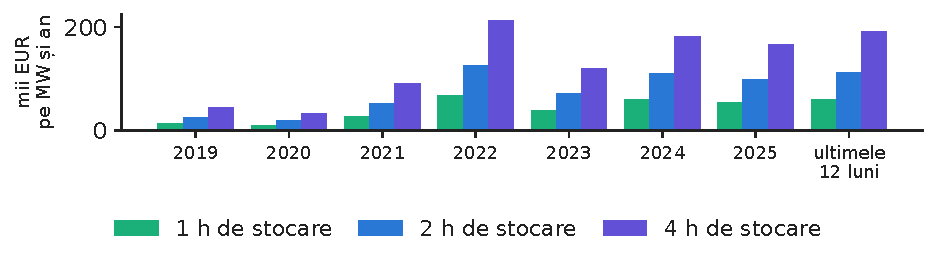
\includegraphics[width=\textwidth,height=0.419\textheight,keepaspectratio]{charts/ro/bat_years.pdf}\end{center}\vspace{-3mm}
\chartsource{Sursa: energy-charts.info; prețuri PZU prin ENTSO-E; producția bateriilor, ENTSO-E (BG, RO); optimizare proprie. Date: 1 MW, randament 85\%, cel mult un ciclu pe zi; 2019-2025 și ultimele 12 luni, 2025-11-01 - 2026-10-31.}
\vspace{0.5mm}
\begin{itemize}\setlength{\itemsep}{0pt}
  \item \textbf{2 ore, mii EUR pe MW și an}: 26{,}3 (2019), 125{,}0 (2022), 98{,}7 (2025)
    \begin{itemize}\setlength{\itemsep}{0pt}
      \item 4 ore cîștigă de 1{,}72 ori cît 2 ore; orele a treia și a patra valorifică o diferență mai mică
    \end{itemize}
\end{itemize}
\par\vfill\manager{dimensionați bateria după venitul adus de fiecare MWh suplimentar de stocare, nu după venitul total.}\par\vspace{0.5mm}
\par\vfill\noindent{\scriptsize\color{FooterGray}(calcule proprii; doar prețurile pentru ziua următoare)}\hfill\qlink{EMQA\_L6\_bat\_years}{Quantlets/L6/EMQA_L6_bat_years}\par\vspace{0.5mm}
\end{frame}

\begin{frame}{O regulă simplă obține 85\% din venitul cu informație perfectă (2 ore)}
\footnotesize
\begin{center}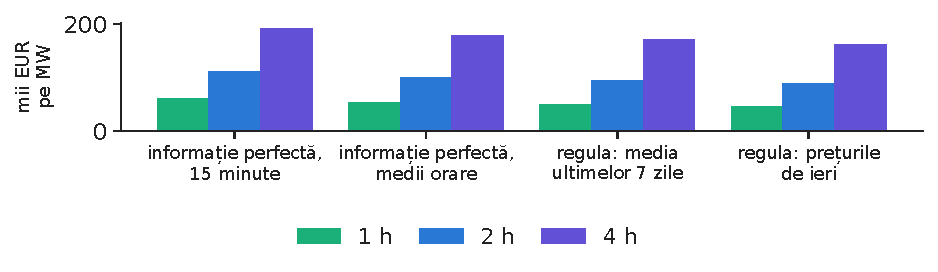
\includegraphics[width=\textwidth,height=0.533\textheight,keepaspectratio]{charts/ro/bat_rules.pdf}\end{center}\vspace{-3mm}
\chartsource{Sursa: energy-charts.info; prețuri PZU prin ENTSO-E; producția bateriilor, ENTSO-E (BG, RO); optimizare proprie. Date: ultimele 12 luni, 2025-11-01 - 2026-10-31; 1 MW, randament 85\%; regulile de prognoză pe 361 de zile comune, scalate la întreaga perioadă.}
\vspace{0.5mm}
\begin{itemize}\setlength{\itemsep}{0pt}
  \item \textbf{Reguli cunoscute la 12:00 CET în ziua $d-1$}: profilul mediu al ultimelor 7 zile, 82\%, 85\%, 89\% (1, 2, 4 ore)
    \begin{itemize}\setlength{\itemsep}{0pt}
      \item Prețurile de ieri: 75\%, 79\%, 84\%; bateriile mai lungi tolerează erorile de sincronizare
    \end{itemize}
\end{itemize}
\par\vfill\manager{bugetați pe baza unei reguli aplicabile: o prognoză mai bună (cursul 2) reduce o parte din diferență.}\par\vspace{0.5mm}
\par\vfill\noindent{\scriptsize\color{FooterGray}(calcule proprii, ultimele 12 luni (noiembrie 2025 -- octombrie 2026))}\hfill\qlink{EMQA\_L6\_bat\_rules}{Quantlets/L6/EMQA_L6_bat_rules}\par\vspace{0.5mm}
\end{frame}

\subsection{Prognoze probabilistice pentru tranzacționare}

\begin{frame}{Prognoza întregii distribuții a prețului ajută o baterie să liciteze}
\footnotesize
\begin{itemize}\setlength{\itemsep}{2pt}
  \item \textbf{Ce a făcut lucrarea}: a prognozat distribuția comună a celor 96 de prețuri orare de a doua zi (24 h $\times$ România, Bulgaria, Ungaria, Cehia)
    \begin{itemize}\setlength{\itemsep}{0pt}
      \item Pădure aleatoare distribuțională, 37 de predictori, ian.\ 2018 -- sep.\ 2024; 70 de ferestre mobile: 365 de zile de estimare, 30 de test
      \item Mediana alege ora de încărcare și ora ulterioară de descărcare; cuantilele fixează prețurile-limită de cumpărare și de vînzare
    \end{itemize}
  \item \textbf{Ce a găsit}: erorile de prognoză sînt maxime la 17:00--18:00, de obicei orele de descărcare
    \begin{itemize}\setlength{\itemsep}{0pt}
      \item România, profitul cumulat al unei baterii de 1 MW / 1 MWh: 143,0 mii EUR cu regula cuantilelor, 133,2 cu ore fixe, 188,2 cu informație perfectă
      \item Regula cuantilelor depășește regula cu ore fixe în toate cele patru piețe; tranzacționarea între piețe adaugă valoare (150,3 mii EUR)
    \end{itemize}
  \item \textbf{Investiția}: la 500\,000 EUR, randament 90\%, 15 ani și 7\%, arbitrajul pe piața pentru ziua următoare nu o acoperă singur
\end{itemize}
\par\vfill\manager{licitați pe baza cuantilelor prognozei, nu a unei singure valori: orele profitabile sînt în cozile distribuției.}\par\vspace{0.5mm}
\par\vfill\noindent{\scriptsize\color{FooterGray}(Andrei, Cepoi, Dumitrescu, Lessmann, Luchian, Pele \& Petukhina, 2026, \href{https://doi.org/10.2139/ssrn.6872381}{doi:10.2139/ssrn.6872381}; prezentarea lui C.\,O.\ Cepoi la AIDA 2026, București, 3 iunie 2026: \href{https://github.com/danpele/EMQA/blob/main/resources/aida2026/cepoi_battery_arbitrage.pdf}{diapozitive})}\par\vspace{0.5mm}
\end{frame}

\subsection{15 minute, autocanibalizare, regiunea}

\begin{frame}{Prețurile pe 15 minute au crescut cu 14{,}5\% venitul unei baterii de 1 oră, în aceleași zile}
\footnotesize
\intuition{Orice program orar poate fi executat pe sferturi de oră, deci prețurile mai fine pot doar să adauge venit.}
\begin{columns}[T,onlytextwidth]
\begin{column}{0.50\textwidth}
\[ R^{15}=\max_{c,x}\textstyle\sum_t P^{15}_t(x_t-c_t)\tfrac14\ \ge\ R^{60} \]{\footnotesize\begin{itemize}\setlength{\itemsep}{0pt}
  \item \textbf{\txtwhere}
    \begin{itemize}\setlength{\itemsep}{0pt}
      \item $R^{15}$ = venitul optim pe cele 96 de prețuri $P^{15}_t$
      \item $R^{60}$ = venitul optim cînd fiecare oră este plătită la media sferturilor ei
      \item Aceleași zile, deci diferența este doar valoarea detalierii.
    \end{itemize}
\end{itemize}\par}
\end{column}
\begin{column}{0.47\textwidth}
\begin{itemize}\setlength{\itemsep}{2pt}
  \item \textbf{Ultimele 12 luni, mii EUR pe MW}
    \begin{itemize}\setlength{\itemsep}{0pt}
      \item 1 oră: 53{,}2 $\to$ 61{,}0 (\ensuremath{+}14{,}5\%)
      \item 2 ore: 100{,}8 $\to$ 111{,}2 (\ensuremath{+}10{,}3\%)
      \item 4 ore: 178{,}4 $\to$ 190{,}9 (\ensuremath{+}7{,}0\%)
    \end{itemize}
  \item O comparație cu anul anterior, orar, ar include și schimbarea nivelului prețurilor.
\end{itemize}
\end{column}
\end{columns}
\par\vfill\manager{bateriile de durată scurtă cîștigă cel mai mult din prețurile pe 15 minute.}\par\vspace{0.5mm}
\par\vfill\noindent{\scriptsize\color{FooterGray}(NEMO Committee, 2025; calcule proprii)}\hfill\tryit{notebook-ul Jupyter, secțiunea 8}\par\vspace{0.5mm}
\end{frame}

\begin{frame}{Bateriile își canibalizează diferența de preț: pe ofertele locale, 50 MW ar fi anulat-o la 21 octombrie 2026}
\footnotesize
\intuition{Încărcarea adaugă cerere la amiază, iar descărcarea adaugă ofertă seara; ambele apropie cele două prețuri.}
\begin{columns}[T,onlytextwidth]
\begin{column}{0.50\textwidth}
\[ \Delta P(X)=p^{*}_{\text{seara}}(+X\text{ ofertă})-p^{*}_{\text{amiază}}(+X\text{ cerere}) \]{\footnotesize\begin{itemize}\setlength{\itemsep}{0pt}
  \item \textbf{\txtwhere}
    \begin{itemize}\setlength{\itemsep}{0pt}
      \item $X$ = puterea bateriilor (MW)
      \item $p^*$ = prețul recalculat pe curbele OPCOM pentru 12:00--12:15 și 20:00--20:15 (ora României)
      \item Fluxuri fixe (Anexa C).
    \end{itemize}
\end{itemize}\par}
\end{column}
\begin{column}{0.47\textwidth}
\begin{itemize}\setlength{\itemsep}{2pt}
  \item \textbf{Prețul de seară minus cel de la amiază}
    \begin{itemize}\setlength{\itemsep}{0pt}
      \item Realizat: 91{,}77 EUR/MWh
      \item 50 MW: \ensuremath{-}13{,}15; 100 MW: \ensuremath{-}47{,}12
    \end{itemize}
  \item \textbf{Baterii deja în funcțiune}
    \begin{itemize}\setlength{\itemsep}{0pt}
      \item România: bateriile au livrat pînă la 766 MW în 2026
      \item Bulgaria (date raportate din 9 septembrie 2026): pînă la 2\,795 MW
    \end{itemize}
\end{itemize}
\end{column}
\end{columns}
\par\vfill\manager{modelați diferența de preț de după construirea bateriilor, nu pe cea observată înainte.}\par\vspace{0.5mm}
\par\vfill\noindent{\scriptsize\color{FooterGray}(curbele agregate OPCOM; calcule proprii)}\hfill\tryit{notebook-ul Jupyter, secțiunea 2}\par\vspace{0.5mm}
\end{frame}

\begin{frame}{O baterie din România concurează pentru aceeași diferență regională de preț ca bateriile din Bulgaria și Ungaria}
\footnotesize
\begin{center}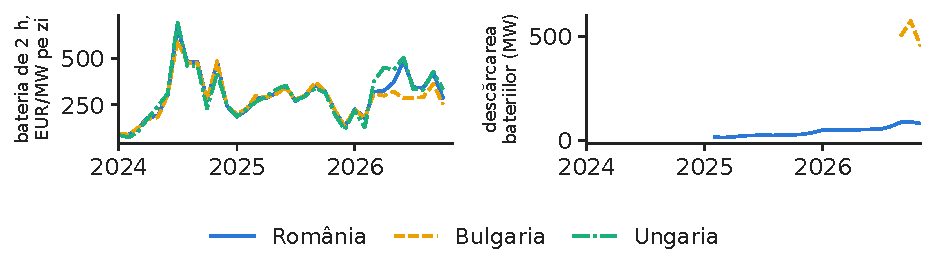
\includegraphics[width=\textwidth,height=0.411\textheight,keepaspectratio]{charts/ro/bat_region.pdf}\end{center}\vspace{-3mm}
\chartsource{Sursa: energy-charts.info; prețuri PZU prin ENTSO-E; producția bateriilor, ENTSO-E (BG, RO); optimizare proprie. Date: baterie de 2 h, informație perfectă, 2024-01 - 2026-10; producția bateriilor raportată la ENTSO-E.}
\vspace{0.5mm}
\begin{itemize}\setlength{\itemsep}{0pt}
  \item \textbf{2 ore, ultimele 12 luni, mii EUR pe MW}: Ungaria 117{,}6, România 111{,}2, Bulgaria 96{,}4, Germania 90{,}6
    \begin{itemize}\setlength{\itemsep}{0pt}
      \item Corelația veniturilor zilnice cu România: Bulgaria 0{,}80, Ungaria 0{,}87
    \end{itemize}
\end{itemize}
\par\vfill\manager{cum am anunțat în cursul 1: un dezvoltator român de baterii concurează pentru aceeași diferență regională de preț de seară.}\par\vspace{0.5mm}
\par\vfill\noindent{\scriptsize\color{FooterGray}(calcule proprii; producția bateriilor raportată la ENTSO-E)}\hfill\qlink{EMQA\_L6\_bat\_region}{Quantlets/L6/EMQA_L6_bat_region}\par\vspace{0.5mm}
\end{frame}

\begin{frame}{La 8\% pe 15 ani, venitul bateriei de 2 ore justifică o investiție de cel mult 808 EUR pe kW}
\footnotesize
\intuition{Investiția maximă pe care o poate recupera un venit anual este venitul înmulțit cu factorul de anuitate.}
\begin{columns}[T,onlytextwidth]
\begin{column}{0.47\textwidth}
\[ I^{\max}=R\cdot a(r,n) \]\[ a(r,n)=\sum_{j=1}^{n}(1+r)^{-j}=\frac{1-(1+r)^{-n}}{r} \]{\footnotesize\begin{itemize}\setlength{\itemsep}{0pt}
  \item \textbf{\txtwhere}
    \begin{itemize}\setlength{\itemsep}{0pt}
      \item $R$ = venitul anual pe MW (EUR), $r$ = 8\% (ipoteză), $n$ = 15 ani (NREL), deci $a$ = 8{,}56
      \item $I^{\max}/1\,000$ = EUR pe kilowatt (kW), Anexa D.
    \end{itemize}
\end{itemize}\par}
\end{column}
\begin{column}{0.50\textwidth}
\begin{itemize}\setlength{\itemsep}{2pt}
  \item \textbf{2 ore, ultimele 12 luni}
    \begin{itemize}\setlength{\itemsep}{0pt}
      \item Informație perfectă: 952 EUR/kW
      \item Regula de 7 zile: 808 EUR/kW = 404 EUR pe kilowatt-oră (kWh)
    \end{itemize}
  \item \textbf{Ce nu am inclus}
    \begin{itemize}\setlength{\itemsep}{0pt}
      \item Costurile de operare, tarifele, pierderea capacității: reduc $I^{\max}$
      \item Veniturile din echilibrare îl cresc; bateriile noi reduc diferența
    \end{itemize}
\end{itemize}
\end{column}
\end{columns}
\par\vfill\manager{comparați 404 EUR/kWh cu oferta pentru instalația la cheie, înaintea oricărei alte analize.}\par\vspace{0.5mm}
\par\vfill\noindent{\scriptsize\color{FooterGray}(Cole \& Karmakar, 2023, NREL; Schmidt et al., 2019, Joule)}\hfill\tryit{notebook-ul Jupyter, secțiunea 8}\par\vspace{0.5mm}
\end{frame}


\section{Studii de caz: aprilie 2026; vara 2026}

\subsection{aprilie 2026: cele mai multe ore cu preț negativ}

\begin{frame}{Studiu de caz: în săptămîna din 20 aprilie 2026, România a avut 24 de ore cu preț negativ, iar rata de captare solară a fost 42\%}
\footnotesize
\begin{center}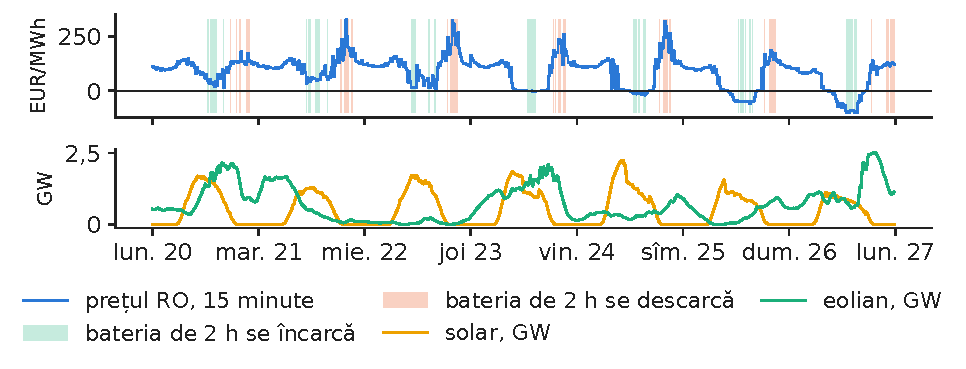
\includegraphics[width=\textwidth,height=0.421\textheight,keepaspectratio]{charts/ro/case_week.pdf}\end{center}\vspace{-3mm}
\chartsource{Sursa: energy-charts.info (Fraunhofer ISE); prețuri OPCOM; producția solară și eoliană și consumul, ENTSO-E (date Transelectrica). Date: săptămîna 2026-04-20 - 2026-04-26, 15 minute, ora CET.}
\vspace{0.5mm}
\begin{itemize}\setlength{\itemsep}{0pt}
  \item \textbf{Prețuri între \ensuremath{-}99{,}75 și 328{,}00 EUR/MWh}; CP solar 37{,}0, față de $B$ 87{,}0
    \begin{itemize}\setlength{\itemsep}{0pt}
      \item Bateria de 2 ore: 391 EUR pe MW pe zi, față de 305 într-o zi medie din ultimele 12 luni
    \end{itemize}
\end{itemize}
\par\vfill\manager{aceeași săptămînă însorită este cea mai slabă pentru un parc solar și una dintre cele mai bune pentru o baterie.}\par\vspace{0.5mm}
\par\vfill\noindent{\scriptsize\color{FooterGray}(calcule proprii; program cu informație perfectă)}\hfill\qlink{EMQA\_L6\_case\_week}{Quantlets/L6/EMQA_L6_case_week}\par\vspace{0.5mm}
\end{frame}

\begin{frame}{Studiu de caz: ce a însemnat luna aprilie 2026 pentru fiecare participant la piață}
\footnotesize
\begin{itemize}\setlength{\itemsep}{3pt}
  \item \textbf{Dezvoltatorul solar}: rata de captare 49{,}4\% (47{,}2 față de 95{,}6 EUR/MWh)
    \begin{itemize}\setlength{\itemsep}{0pt}
      \item 17{,}9\% din producție la prețuri negative; decizie: stocare în același amplasament sau un PPA care stabilește prețul profilului solar
    \end{itemize}
  \item \textbf{Dezvoltatorul eolian}: rata de captare 97{,}8\%
    \begin{itemize}\setlength{\itemsep}{0pt}
      \item În România, eolianul nu este tehnologia canibalizată
    \end{itemize}
  \item \textbf{Dezvoltatorul de baterii}: 2 ore, 325 EUR pe MW pe zi
    \begin{itemize}\setlength{\itemsep}{0pt}
      \item Față de 305 în medie în ultimele 12 luni
    \end{itemize}
  \item \textbf{Furnizorul și consumatorul industrial}: 67 de ore cu preț negativ
    \begin{itemize}\setlength{\itemsep}{0pt}
      \item Mutarea consumului la amiază, primăvara, este plătită
    \end{itemize}
  \item \textbf{Transelectrica}
    \begin{itemize}\setlength{\itemsep}{0pt}
      \item După apus, creșterea cererii nete și interconexiunile fixează prețul
    \end{itemize}
\end{itemize}
\par\vfill\noindent{\scriptsize\color{FooterGray}(calcule proprii)}\hfill\tryit{notebook-ul Jupyter, secțiunea 9}\par\vspace{0.5mm}
\end{frame}

\subsection{Vara 2026: România și Bulgaria}

\begin{frame}{Vara 2026: export la prînz, import seara din Bulgaria}
\footnotesize
\begin{center}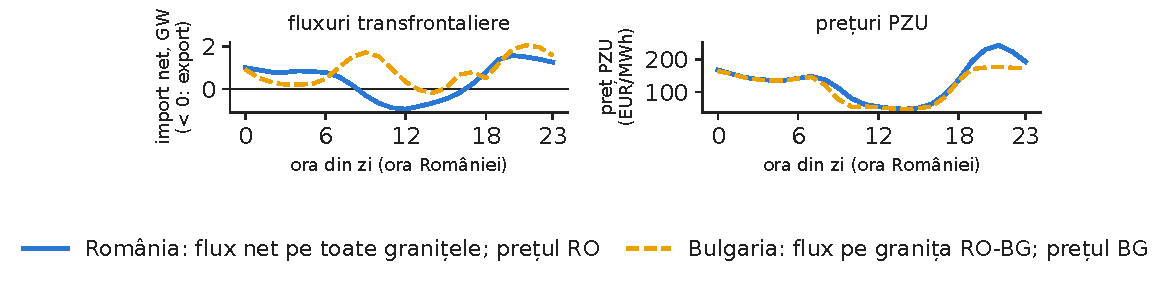
\includegraphics[width=\textwidth,height=0.425\textheight,keepaspectratio]{charts/ro/rogb_summer.pdf}\end{center}\vspace{-3mm}
\chartsource{Sursa: energy-charts.info (Fraunhofer ISE): fluxurile fizice transfrontaliere ale României (ENTSO-E); prețurile pentru ziua următoare OPCOM (RO) și IBEX (BG). Date: medii orare, 2026-06-01 - 2026-08-31; granițele cu Moldova și Ucraina sînt raportate doar parțial.}
\vspace{0.5mm}
\begin{itemize}\setlength{\itemsep}{0pt}
  \item \textbf{La prînz România exportă}: 960 MW net la ora 12, pe toate granițele
    \begin{itemize}\setlength{\itemsep}{0pt}
      \item Mai ales spre Ungaria (857 MW) și Serbia (367 MW); spre Bulgaria doar în 43 din 92 de zile (12:00--15:00)
    \end{itemize}
  \item \textbf{Seara România importă din Bulgaria}: 2\,064 MW la ora 21, în toate cele 92 de zile
    \begin{itemize}\setlength{\itemsep}{0pt}
      \item Prețul la ora 21: România 243{,}9, Bulgaria 178{,}3 EUR/MWh; granița plină separă cele două prețuri
    \end{itemize}
\end{itemize}
\par\vfill\manager{diferența de seară, de 65{,}6 EUR/MWh, este valoarea stocării de seară și a interconexiunii.}\par\vspace{0.5mm}
\par\vfill\noindent{\scriptsize\color{FooterGray}(calcule proprii; + = import în România)}\hfill\qlink{EMQA\_L6\_rogb\_summer}{Quantlets/L6/EMQA_L6_rogb_summer}\par\vspace{0.5mm}
\end{frame}

\section*{Recapitulare}

\begin{frame}{Test 1: rata de captare}
\small
\begin{itemize}
  \item Vi se oferă un PPA solar la prețul de bază din 2025, de 108 EUR/MWh
    \begin{itemize}\setlength{\itemsep}{0pt}
      \item Cît obține de fapt profilul solar?
    \end{itemize}
\end{itemize}
\vspace{2mm}
\begin{exampleblock}{R\u{a}spuns}
\begin{itemize}
  \item Aproximativ 64 EUR/MWh în 2025 (rata de captare 59\%)
    \begin{itemize}\setlength{\itemsep}{0pt}
      \item Cumpărătorul care plătește prețul de bază plătește o primă mare pentru profil.
    \end{itemize}
\end{itemize}
\end{exampleblock}
\end{frame}

\begin{frame}{Test 2: numărarea prețurilor negative}
\small
\begin{itemize}
  \item De la 1 octombrie 2025, România a avut 687 de sferturi de oră cu preț negativ
    \begin{itemize}\setlength{\itemsep}{0pt}
      \item Cîte ore cu preț negativ raportați?
    \end{itemize}
\end{itemize}
\vspace{2mm}
\begin{exampleblock}{R\u{a}spuns}
\begin{itemize}
  \item 171{,}75 ore echivalente (fiecare sfert de oră contează 0{,}25 h), nu 687 de ore.
\end{itemize}
\end{exampleblock}
\end{frame}

\begin{frame}{Test 3: durata bateriei}
\small
\begin{itemize}
  \item Dublarea stocării de la 2 la 4 ore dublează costul celulelor
    \begin{itemize}\setlength{\itemsep}{0pt}
      \item Se dublează și venitul?
    \end{itemize}
\end{itemize}
\vspace{2mm}
\begin{exampleblock}{R\u{a}spuns}
\begin{itemize}
  \item Nu
    \begin{itemize}\setlength{\itemsep}{0pt}
      \item În ultimele 12 luni, o baterie de 4 ore a cîștigat de 1{,}72 ori cît una de 2 ore, deoarece orele suplimentare valorifică o diferență de preț mai mică.
    \end{itemize}
\end{itemize}
\end{exampleblock}
\end{frame}

\begin{frame}{Test 4: efectul ordinii de merit}
\small
\begin{itemize}
  \item Pe curbele OPCOM din 21 octombrie 2026, 25 MW în plus la preț zero coboară prețul de la amiază la 131{,}4 EUR/MWh
    \begin{itemize}\setlength{\itemsep}{0pt}
      \item Acesta este efectul unui parc nou de 25 MW?
    \end{itemize}
\end{itemize}
\vspace{2mm}
\begin{exampleblock}{R\u{a}spuns}
\begin{itemize}
  \item Nu
    \begin{itemize}\setlength{\itemsep}{0pt}
      \item Curbele păstrează fixe fluxurile transfrontaliere, iar în piața cuplată o parte din producție se exportă, deci efectul real este mai mic (regresia dă o scădere de aproximativ 27 EUR/MWh pentru fiecare GW).
    \end{itemize}
\end{itemize}
\end{exampleblock}
\end{frame}

\begin{frame}{Recapitulare}
\small
\vspace{-2mm}\begin{multicols}{2}\scriptsize\tableofcontents\end{multicols}
\begin{itemize}\setlength{\itemsep}{1pt}
  \item Producția solară reduce prețul pe care îl primește
    \begin{itemize}\setlength{\itemsep}{0pt}
      \item Rata de captare în România: 104\% (2019) $\to$ 59\% (2025)
      \item Eolianul rămîne aproape de 100\%.
    \end{itemize}
  \item Bateriile trăiesc din aceeași diferență regională de preț
    \begin{itemize}\setlength{\itemsep}{0pt}
      \item 111 mii EUR pe MW pentru 2 ore, cu informație perfectă, și circa 85\% din această sumă cu o regulă simplă
      \item Urmează cursul 7.
    \end{itemize}
\end{itemize}
\end{frame}

\begin{frame}{Cercetările grupului nostru despre sursele regenerabile și prețurile din România}
\footnotesize
\begin{itemize}\setlength{\itemsep}{2pt}
  \item \textbf{Explicarea scăderilor și salturilor de preț} (Andrei \& Pele, 2025, Preprints)
    \begin{itemize}\setlength{\itemsep}{0pt}
      \item Ce a făcut lucrarea: a identificat prețurile orare neobișnuite din România cu algoritmul isolation forest și le-a explicat cu valori Shapley
      \item Rezultat: producția eoliană și cea solară explică scăderile de preț; erorile de prognoză a consumului și producția convențională explică salturile
    \end{itemize}
  \item \textbf{Factorii prețului pe orizonturi și regimuri} (Andrei, Pele \& Cramer, 2026, PICBE)
    \begin{itemize}\setlength{\itemsep}{0pt}
      \item Ce a făcut lucrarea: a prognozat prețurile orare din România în perioada 2018--2024 cu ansambluri de arbori și a măsurat ce factori contează la fiecare orizont și în regimurile de preț scăzut, normal și ridicat
      \item Legătura cu acest curs: factorii regenerabili din spatele regimului de preț scăzut
    \end{itemize}
  \item \textbf{Avertizarea timpurie a salturilor de preț} (Andrei, Pele, Cramer, Amza \& Diaconu, 2026, PICBE)
    \begin{itemize}\setlength{\itemsep}{0pt}
      \item Ce a făcut lucrarea: a construit un sistem explicabil de inteligență artificială (AI) pentru avertizarea timpurie a salturilor de preț din România
      \item Rezultat: prognoza consumului rezidual este principalul factor, aceeași variabilă ca în regresia noastră
    \end{itemize}
  \item \textbf{Elasticitatea cererii de energie electrică} (Proșcanu, Proșcanu \& Pele, 2025, JSES)
    \begin{itemize}\setlength{\itemsep}{0pt}
      \item Ce a făcut lucrarea: a testat cauzalitatea Granger între consumul și prețul energiei electrice din România
      \item Rezultat: consumul nu reacționează la preț, de aici curba cererii aproape verticală din ordinea de merit
    \end{itemize}
\end{itemize}
\par\vspace{0.5mm}{\scriptsize \begin{itemize}\setlength{\itemsep}{0pt}
  \item Rezultatele de pe acest diapozitiv sînt cele raportate în lucrări; celelalte cifre din curs provin din calculele noastre.
\end{itemize}}
\par\vfill\noindent{\scriptsize\color{FooterGray}(Academia de Studii Economice din București; Academia Română, Institutul de Prognoză Economică)}\par\vspace{0.5mm}
\end{frame}

\begin{frame}{Lecturi și resurse suplimentare}
\small
\begin{columns}[T,onlytextwidth]
\begin{column}{0.52\textwidth}
\begin{itemize}\setlength{\itemsep}{4pt}
  \item \textbf{Hirth (2013)}: lucrarea de referință despre rata de captare a energiei eoliene și solare: \href{https://doi.org/10.1016/j.eneco.2013.02.004}{doi:10.1016/j.eneco.2013.02.004}.
  \item \textbf{Cole \& Karmakar (2023)}: costurile, randamentul și durata de viață a bateriilor, folosite în acest curs: \href{https://doi.org/10.2172/1984976}{doi:10.2172/1984976}.
  \item \textbf{energy-charts.info}: prețuri, producție și putere instalată, actualizate, pentru România și vecinii ei: \href{https://energy-charts.info}{energy-charts.info}.
\end{itemize}
\end{column}
\begin{column}{0.45\textwidth}
\begin{itemize}\setlength{\itemsep}{4pt}
  \item \textbf{Acest curs}: cod, date, notebook-uri Jupyter --- \href{https://github.com/danpele/EMQA}{github.com/danpele/EMQA}.
  \item \textbf{Curbele agregate OPCOM}: descărcați altă zi și repetați calculul ordinii de merit: \href{https://www.opcom.ro/rapoarte-pzu-curbe-agregate/ro}{opcom.ro}.
  \item \textbf{Exercițiu practic}: notebook-ul Jupyter reproduce toate graficele și cifrele din acest curs.
\end{itemize}
\end{column}
\end{columns}
\end{frame}

\begin{frame}{Bibliografie (1/3)}
\scriptsize
\begin{itemize}\setlength{\itemsep}{1pt}\scriptsize
\item Andrei, A.-V.\ \& Pele, D.\,T.\ (2025). Explainable AI for electricity price anomaly detection: A SHAP-driven approach in Romania's energy market. \textit{Preprints}. \href{https://doi.org/10.20944/preprints202508.0410.v1}{doi:10.20944/preprints202508.0410.v1}
\item Andrei, A.-V., Cepoi, C., Dumitrescu, B.-A., Lessmann, S., Luchian, A., Pele, D.-T.\ \& Petukhina, A.\ (2026). Joint probabilistic forecasting for battery arbitrage in day-ahead power markets. SSRN Working Paper 6872381. \href{https://doi.org/10.2139/ssrn.6872381}{doi:10.2139/ssrn.6872381}
\item Andrei, A.-V., Pele, D.-T.\ \& Cramer, A.-A.\ (2026). Multi-horizon explainability in energy price forecasting: Disentangling market dynamics and renewable intermittency in Romania's liberalized electricity market. \textit{Proceedings of the International Conference on Business Excellence}, 20(1), 104--117. \href{https://doi.org/10.2478/picbe-2026-0014}{doi:10.2478/picbe-2026-0014}
\item Andrei, A.-V., Pele, D.-T., Cramer, A.-A., Amza, A.\ \& Diaconu, D.\ (2026). Explainable AI-based early warning system for electricity price spikes: Evidence from the Romanian market. \textit{Proceedings of the International Conference on Business Excellence}, 20(1), 4820--4836. \href{https://doi.org/10.2478/picbe-2026-0352}{doi:10.2478/picbe-2026-0352}
\item Basangova, M., Bolovăneanu, V., Conda, A., Erlwein-Sayer, C., Melzer, A., Pele, D.\,T., Petukhina, A.\ \& Phan, M.\ (2026). Day-ahead forecasting for redispatch measures using machine learning models. Talk at the AIDA Conference, Bucharest University of Economic Studies, 3 June 2026. \href{https://github.com/danpele/EMQA/blob/main/resources/aida2026/bolovaneanu_redispatch_forecasting.pdf}{github.com/danpele/EMQA}
\item Bradbury, K., Pratson, L.\ \& Patiño-Echeverri, D.\ (2014). Economic viability of energy storage systems based on price arbitrage potential in real-time U.S.\ electricity markets. \textit{Applied Energy}, 114, 512--519. \href{https://doi.org/10.1016/j.apenergy.2013.10.010}{doi:10.1016/j.apenergy.2013.10.010}
\item Cludius, J., Hermann, H., Matthes, F.\,C.\ \& Graichen, V.\ (2014). The merit order effect of wind and photovoltaic electricity generation in Germany 2008--2016: Estimation and distributional implications. \textit{Energy Economics}, 44, 302--313. \href{https://doi.org/10.1016/j.eneco.2014.04.020}{doi:10.1016/j.eneco.2014.04.020}
\end{itemize}
\end{frame}

\begin{frame}{Bibliografie (2/3)}
\scriptsize
\begin{itemize}\setlength{\itemsep}{1pt}\scriptsize
\item Cepoi, C.\,O.\ (2026). Uncertainty meets opportunity: Joint probabilistic forecasting for battery arbitrage in CEE day-ahead power markets. Talk at the AIDA Conference, Bucharest University of Economic Studies, 3 June 2026. \href{https://github.com/danpele/EMQA/blob/main/resources/aida2026/cepoi_battery_arbitrage.pdf}{github.com/danpele/EMQA}
\item Cole, W.\ \& Karmakar, A.\ (2023). Cost projections for utility-scale battery storage: 2023 update. NREL/TP-6A40-85332, National Renewable Energy Laboratory. \href{https://doi.org/10.2172/1984976}{doi:10.2172/1984976}
\item Fanone, E., Gamba, A.\ \& Prokopczuk, M.\ (2013). The case of negative day-ahead electricity prices. \textit{Energy Economics}, 35, 22--34. \href{https://doi.org/10.1016/j.eneco.2011.12.006}{doi:10.1016/j.eneco.2011.12.006}
\item Hirth, L.\ (2013). The market value of variable renewables: The effect of solar wind power variability on their relative price. \textit{Energy Economics}, 38, 218--236. \href{https://doi.org/10.1016/j.eneco.2013.02.004}{doi:10.1016/j.eneco.2013.02.004}
\item Hirth, L., Ueckerdt, F.\ \& Edenhofer, O.\ (2016). Why wind is not coal: On the economics of electricity generation. \textit{The Energy Journal}, 37(3), 1--28. \href{https://doi.org/10.5547/01956574.37.3.lhir}{doi:10.5547/01956574.37.3.lhir}
\item López Prol, J., Steininger, K.\,W.\ \& Zilberman, D.\ (2020). The cannibalization effect of wind and solar in the California wholesale electricity market. \textit{Energy Economics}, 85, 104552. \href{https://doi.org/10.1016/j.eneco.2019.104552}{doi:10.1016/j.eneco.2019.104552}
\item NEMO Committee (2025). 15-Minute MTU in SDAC was implemented. Single Day-Ahead Coupling (SDAC) press release, 1 October 2025. \href{https://nemo-committee.eu/assets/files/15-minute-mtu-in-sdac-was-implemented.pdf}{nemo-committee.eu}
\end{itemize}
\end{frame}

\begin{frame}{Bibliografie (3/3)}
\scriptsize
\begin{itemize}\setlength{\itemsep}{1pt}\scriptsize
\item Proșcanu, C., Proșcanu, M.\ \& Pele, D.\,T.\ (2025). The price elasticity of electricity demand in Romania. \textit{Journal of Social and Economic Statistics}, 14(2), 131--141. \href{https://doi.org/10.2478/jses-2025-0009}{doi:10.2478/jses-2025-0009}
\item Schmidt, O., Melchior, S., Hawkes, A.\ \& Staffell, I.\ (2019). Projecting the future levelized cost of electricity storage technologies. \textit{Joule}, 3(1), 81--100. \href{https://doi.org/10.1016/j.joule.2018.12.008}{doi:10.1016/j.joule.2018.12.008}
\item Sensfuß, F., Ragwitz, M.\ \& Genoese, M.\ (2008). The merit-order effect: A detailed analysis of the price effect of renewable electricity generation on spot market prices in Germany. \textit{Energy Policy}, 36(8), 3086--3094. \href{https://doi.org/10.1016/j.enpol.2008.03.035}{doi:10.1016/j.enpol.2008.03.035}
\item Sioshansi, R., Denholm, P., Jenkin, T.\ \& Weiss, J.\ (2009). Estimating the value of electricity storage in PJM: Arbitrage and some welfare effects. \textit{Energy Economics}, 31(2), 269--277. \href{https://doi.org/10.1016/j.eneco.2008.10.005}{doi:10.1016/j.eneco.2008.10.005}
\item Weron, R.\ (2014). Electricity price forecasting: A review of the state-of-the-art with a look into the future. \textit{International Journal of Forecasting}, 30(4), 1030--1081. \href{https://doi.org/10.1016/j.ijforecast.2014.08.008}{doi:10.1016/j.ijforecast.2014.08.008}
\item Würzburg, K., Labandeira, X.\ \& Linares, P.\ (2013). Renewable generation and electricity prices: Taking stock and new evidence for Germany and Austria. \textit{Energy Economics}, 40, S159--S171. \href{https://doi.org/10.1016/j.eneco.2013.09.011}{doi:10.1016/j.eneco.2013.09.011}
\end{itemize}
\end{frame}

\appendix

\section*{Anexă}

\begin{frame}{Anexa A: rata de captare este unu plus o covarianță scalată}
\footnotesize
\begin{itemize}\setlength{\itemsep}{3pt}
  \item \textbf{Notație}
    \begin{itemize}\setlength{\itemsep}{0pt}
      \item Ponderile $w_t=\Delta_t/\sum_s\Delta_s$; $\bar P=\sum_t w_tP_t=B$; $\bar G=\sum_t w_tG_t$; $\mathrm{Cov}_\Delta(P,G)=\sum_t w_t(P_t-\bar P)(G_t-\bar G)$
    \end{itemize}
  \item \textbf{Pasul 1}
    \begin{itemize}\setlength{\itemsep}{0pt}
      \item Se împart numărătorul și numitorul lui CP la $\sum_s\Delta_s$: $\mathrm{CP}=\sum_t w_tP_tG_t\,/\,\bar G$
    \end{itemize}
  \item \textbf{Pasul 2}
    \begin{itemize}\setlength{\itemsep}{0pt}
      \item $\sum_t w_tP_tG_t=\mathrm{Cov}_\Delta(P,G)+\bar P\bar G$ (definiția covarianței)
    \end{itemize}
  \item \textbf{Pasul 3}
    \begin{itemize}\setlength{\itemsep}{0pt}
      \item $\mathrm{CR}=\mathrm{CP}/\bar P=1+\mathrm{Cov}_\Delta(P,G)/(\bar P\bar G)$
      \item Producția solară din România, ian.--oct. 2026: $\bar P$ = 137{,}4, $\bar G$ = 593 MW, covarianța \ensuremath{-}31\,069, deci CR = 0{,}619
    \end{itemize}
  \item \textbf{Interpretare}
    \begin{itemize}\setlength{\itemsep}{0pt}
      \item CR $<1$ exact atunci cînd producția este mare în intervalele ieftine; CR nu este definită dacă $\bar P\le 0$
    \end{itemize}
\end{itemize}
\par\vfill\noindent{\scriptsize\color{FooterGray}(Hirth, 2013, ENEECO)}\par\vspace{0.5mm}
\end{frame}

\begin{frame}{Anexa B: programul bateriei în formă matriceală}
\footnotesize
\begin{itemize}\setlength{\itemsep}{3pt}
  \item \textbf{Variabile}
    \begin{itemize}\setlength{\itemsep}{0pt}
      \item $z=(c_1..c_T,\,x_1..x_T,\,e_1..e_T)$, $3T$ variabile; $T$ = 92, 96 sau 100 de sferturi de oră (24 de ore înainte de octombrie 2025)
    \end{itemize}
  \item \textbf{Funcția obiectiv}
    \begin{itemize}\setlength{\itemsep}{0pt}
      \item Se minimizează $\sum_t P_t\Delta_t c_t-\sum_t P_t\Delta_t x_t$ (venitul cu semn schimbat)
    \end{itemize}
  \item \textbf{Egalități}
    \begin{itemize}\setlength{\itemsep}{0pt}
      \item $e_t-e_{t-1}-\sqrt\eta\Delta_tc_t+\Delta_tx_t/\sqrt\eta=0$ pentru $t=1..T$, cu $e_0=0$; în plus, $e_T=0$
    \end{itemize}
  \item \textbf{Inegalitate și limite}
    \begin{itemize}\setlength{\itemsep}{0pt}
      \item $\sum_t\Delta_tx_t/\sqrt\eta\le E$; $0\le c_t,x_t\le1$; $0\le e_t\le E$; rezolvare cu algoritmul HiGHS (scipy)
    \end{itemize}
  \item \textbf{Regulile de prognoză}
    \begin{itemize}\setlength{\itemsep}{0pt}
      \item Programul se rezolvă pe $\hat P_t$ (media ultimelor 7 zile sau prețurile zilei $d-1$), apoi venitul este $\sum_tP_t(x_t-c_t)\Delta_t$, cu prețurile reale $P_t$
      \item Zilele cu alt număr de intervale decît prognoza (schimbarea orei) sînt eliminate: rămîn 361 din 365 zile
    \end{itemize}
\end{itemize}
\par\vfill\noindent{\scriptsize\color{FooterGray}(Sioshansi et al., 2009, ENEECO)}\par\vspace{0.5mm}
\end{frame}

\begin{frame}{Anexa C: recalcularea prețului de închidere pe curbele OPCOM}
\footnotesize
\begin{itemize}\setlength{\itemsep}{3pt}
  \item \textbf{Curbele}
    \begin{itemize}\setlength{\itemsep}{0pt}
      \item OPCOM publică, pentru fiecare sfert de oră, punctele agregate ale ofertei și cererii (preț, MW cumulați), în format XML
      \item Blocurile, ordinele orare și fluxurile transfrontaliere nete se adaugă la limitele de preț ($-$600 și $+$4\,000 EUR/MWh), ca în graficul OPCOM
    \end{itemize}
  \item \textbf{Algoritmul}
    \begin{itemize}\setlength{\itemsep}{0pt}
      \item $S(p)$, $D(p)$ = interpolare liniară între punctele publicate; noul preț = cel mai mic $p$ pentru care $S(p)+X\mathbf 1[p\ge0]-D(p)\ge0$, găsit prin bisecție pe $[-600,4000]$
      \item Pentru încărcarea bateriilor, se adaugă la $D$ cererea de $X$ MW la orice preț
    \end{itemize}
  \item \textbf{Verificare}
    \begin{itemize}\setlength{\itemsep}{0pt}
      \item Pentru $X=0$, curbele se intersectează pe un segment orizontal: la amiază de la 152{,}16 în sus, seara de la 206{,}49; prețurile oficiale 152{,}23 și 244{,}00 se află pe aceste segmente
      \item Pentru $X=0$ folosim prețul oficial
    \end{itemize}
\end{itemize}
\par\vfill\noindent{\scriptsize\color{FooterGray}(OPCOM; data/clean/opcom\_pzu\_curves\_meta.json)}\par\vspace{0.5mm}
\end{frame}

\begin{frame}{Anexa D: factorul de anuitate}
\footnotesize
\begin{itemize}\setlength{\itemsep}{3pt}
  \item \textbf{Valoarea actualizată a unui venit constant}
    \begin{itemize}\setlength{\itemsep}{0pt}
      \item $V=\sum_{j=1}^{n}R(1+r)^{-j}=R\,q\,\frac{1-q^{n}}{1-q}$, cu $q=(1+r)^{-1}$
    \end{itemize}
  \item \textbf{Simplificare}
    \begin{itemize}\setlength{\itemsep}{0pt}
      \item $q/(1-q)=1/r$, deci $V=R\,\frac{1-(1+r)^{-n}}{r}=R\,a(r,n)$
    \end{itemize}
  \item \textbf{Pragul de rentabilitate}
    \begin{itemize}\setlength{\itemsep}{0pt}
      \item Proiectul se recuperează dacă investiția $I\le V$; pentru $r$ = 8\% și $n$ = 15: $a$ = 8{,}56
    \end{itemize}
  \item \textbf{Pe kWh de stocare}
    \begin{itemize}\setlength{\itemsep}{0pt}
      \item $I^{\max}/E$: pentru 1, 2 și 4 ore, cu regula de 7 zile, 428, 404 și 365 EUR/kWh
    \end{itemize}
\end{itemize}
\par\vfill\noindent{\scriptsize\color{FooterGray}(Cole \& Karmakar, 2023, NREL)}\par\vspace{0.5mm}
\end{frame}

\end{document}
